% !TeX root = main.tex

\documentclass[
% -- opções da classe memoir --
12pt,				% tamanho da fonte
openany,			% capítulos iniciam na próxima pág disponível (sem inserir páginas em branco)
oneside,			% para impressão em recto e verso. Oposto a oneside
a4paper,			% tamanho do papel. 
% -- opções da classe abntex2 --
%chapter=TITLE,		% títulos de capítulos convertidos em letras maiúsculas
%section=TITLE,		% títulos de seções convertidos em letras maiúsculas
%subsection=TITLE,	% títulos de subseções convertidos em letras maiúsculas
%subsubsection=TITLE,% títulos de subsubseções convertidos em letras maiúsculas
% -- opções do pacote babel --
english,			% idioma adicional para hifenização
french,				% idioma adicional para hifenização
spanish,			% idioma adicional para hifenização
brazil				% o último idioma é o principal do documento
]{abntex2}

% ---
% Pacotes básicos 
% ---
\usepackage{lmodern}			% Usa a fonte Latin Modern			
\usepackage[T1]{fontenc}		% Selecao de codigos de fonte.
\usepackage[utf8]{inputenc}		% Codificacao do documento (conversão automática dos acentos)
\usepackage{indentfirst}		% Indenta o primeiro parágrafo de cada seção.
\usepackage{color}				% Controle das cores
\usepackage{graphicx}			% Inclusão de gráficos
\usepackage{microtype} 			% para melhorias de justificação
% ---

% ---
% Pacotes adicionais, usados apenas no âmbito do Modelo Canônico do abnteX2
% ---
\usepackage{lipsum}				% para geração de dummy text
% ---
\usepackage{amssymb}   %para checkmark
% ---
% Pacotes de citações
% ---
\usepackage[brazilian,hyperpageref]{backref}	 % Paginas com as citações na bibl
\usepackage[alf]{abntex2cite}	% Citações padrão ABNT
% ---
% Pacotes adicionados pelos autores
% ---
\usepackage{enumitem}							% para personalizar listas numeradas
\usepackage{qrcode}								% para gerar QR code
\usepackage{longtable}         					%para tabelas longas
\usepackage[section]{placeins} % para barreiras

% --- 
% CONFIGURAÇÕES DE PACOTES
% ---

% Configurações do pacote backref
% Usado sem a opção hyperpageref de backref
\renewcommand{\backrefpagesname}{Citado na(s) página(s):~}
% Texto padrão antes do número das páginas
\renewcommand{\backref}{}
% Define os textos da citação
\renewcommand*{\backrefalt}[4]{
	\ifcase #1 %
	Nenhuma citação no texto.%
	\or
	Citado na página #2.%
	\else
	Citado #1 vezes nas páginas #2.%
	\fi}%

% Configuração do pacote enumitem
% Aplicando o recuo em listas numeradas globalmente
\setlist[enumerate]{leftmargin=2cm}
% ---

% ---
% Informações de dados para CAPA e FOLHA DE ROSTO
% ---
\titulo{Projeto Integrado de Extensão I}
\autor{BS Beauty Academy}
\local{São Paulo, SP - Brasil}
\data{2025}
\orientador{Marcelo Tavares}
\instituicao{%
	Instituto Federal de Educação, Ciência e\\ Tecnologia de São Paulo -- IFSP
	\par
	Tecnologia em Análise e Desenvolvimento de Sistemas
	\par
	Programa de graduação}
\tipotrabalho{Projeto Integrado de Extensão}
% O preambulo deve conter o tipo do trabalho, o objetivo, 
% o nome da instituição e a área de concentração 
\preambulo{Este projeto integrado de extensão, desenvolvido como parte do curso de Tecnologia em Análise e Desenvolvimento de Sistemas do Instituto Federal de Educação, Ciência e Tecnologia de São Paulo, tem como objetivo desenvolver uma aplicação web para otimizar a gestão e o agendamento de serviços de estética em um ambiente coworking. A área de concentração do projeto é a inovação tecnológica aplicada ao setor de serviços de beleza.}
% ---

% Configurações de aparência do PDF final

% alterando o aspecto da cor azul
\definecolor{blue}{RGB}{41,5,195}

% informações do PDF
\makeatletter
\hypersetup{
	%pagebackref=true,
	pdftitle={\@title}, 
	pdfauthor={\@author},
	pdfsubject={\imprimirpreambulo},
	pdfcreator={LaTeX with abnTeX2},
	pdfkeywords={abnt}{latex}{abntex}{abntex2}{trabalho acadêmico}, 
	colorlinks=true,       		% false: boxed links; true: colored links
	linkcolor=blue,          	% color of internal links
	citecolor=blue,        		% color of links to bibliography
	filecolor=magenta,      		% color of file links
	urlcolor=blue,
	bookmarksdepth=4
}
\makeatother
% --- 

% ---
% Posiciona figuras e tabelas no topo da página quando adicionadas sozinhas
% em um página em branco. Ver https://github.com/abntex/abntex2/issues/170
\makeatletter
\setlength{\@fptop}{5pt} % Set distance from top of page to first float
\makeatother
% ---

% ---
% Possibilita criação de Quadros e Lista de quadros.
% Ver https://github.com/abntex/abntex2/issues/176
%
\newcommand{\quadroname}{Quadro}
\newcommand{\listofquadrosname}{Lista de quadros}

\newfloat[chapter]{quadro}{loq}{\quadroname}
\newlistof{listofquadros}{loq}{\listofquadrosname}
\newlistentry{quadro}{loq}{0}

% configurações para atender às regras da ABNT
\setfloatadjustment{quadro}{\centering}
\counterwithout{quadro}{chapter}
\renewcommand{\cftquadroname}{\quadroname\space} 
\renewcommand*{\cftquadroaftersnum}{\hfill--\hfill}

\setfloatlocations{quadro}{hbtp} % Ver https://github.com/abntex/abntex2/issues/176
% ---

% --- 
% Espaçamentos entre linhas e parágrafos 
% --- 

% O tamanho do parágrafo é dado por:
\setlength{\parindent}{1.3cm}

% Controle do espaçamento entre um parágrafo e outro:
\setlength{\parskip}{0.2cm}  % tente também \onelineskip

% ---
% compila o indice
% ---
\makeindex
% ---

% ----
% Início do documento
% ----
\begin{document}
	
	% Seleciona o idioma do documento (conforme pacotes do babel)
	%\selectlanguage{english}
	\selectlanguage{brazil}
	
	% Retira espaço extra obsoleto entre as frases.
	\frenchspacing 
	
	% ----------------------------------------------------------
	% ELEMENTOS PRÉ-TEXTUAIS
	% ----------------------------------------------------------
	% \pretextual
	
	% ---
	% Capa
	% ---
	\imprimircapa
	% ---
	
	% ---
	% Folha de rosto
	% (o * indica que haverá a ficha bibliográfica)
	% ---
	\imprimirfolhaderosto*
	% ---
	
	% ---
	% Inserir a ficha bibliografica
	% ---
	
	% Isto é um exemplo de Ficha Catalográfica, ou ``Dados internacionais de
	% catalogação-na-publicação''. Você pode utilizar este modelo como referência. 
	% Porém, provavelmente a biblioteca da sua universidade lhe fornecerá um PDF
	% com a ficha catalográfica definitiva após a defesa do trabalho. Quando estiver
	% com o documento, salve-o como PDF no diretório do seu projeto e substitua todo
	% o conteúdo de implementação deste arquivo pelo comando abaixo:
	%
	% \begin{fichacatalografica}
		%     \includepdf{fig_ficha_catalografica.pdf}
		% \end{fichacatalografica}
	
	\begin{fichacatalografica}
		\sffamily
		\vspace*{\fill}					% Posição vertical
		\begin{center}					% Minipage Centralizado
			\fbox{\begin{minipage}[c][8cm]{13.5cm}		% Largura
					\small
					\imprimirautor
					%Sobrenome, Nome do autor
					
					\hspace{0.5cm} \imprimirtitulo  / \imprimirautor. --
					\imprimirlocal, \imprimirdata
					
					\hspace{0.5cm} \thelastpage p. : il. color; 30cm 
					
					\hspace{0.5cm} \imprimirorientadorRotulo~\imprimirorientador\\
					
					\hspace{0.5cm}
					\parbox[t]{\textwidth}{\imprimirtipotrabalho~--~\imprimirinstituicao,
						\imprimirdata.}\\
					
					\hspace{0.5cm}
					1. Graduação
					2. Extensão
					3. Integrado \\
					I. Marcelo Tavares.
					II. IFSP.
					III. Análise e Desenvolvimento de Sistemas. 
					IV. PIE1 			
			\end{minipage}}
		\end{center}
	\end{fichacatalografica}
	% ---
	
	% ---
	% Inserir errata
	% ---
	\begin{errata}
		pagina opcional para descrever algum correção que deve ser feita no documento.
		
		\begin{table}[htb]
			\center
			\footnotesize
			\begin{tabular}{|p{1.4cm}|p{1cm}|p{3cm}|p{3cm}|}
				\hline
				\textbf{Folha} & \textbf{Linha}  & \textbf{Onde se lê}  & \textbf{Leia-se}  \\
				\hline
				1 & 10 & auto-conclavo & autoconclavo\\
				\hline
			\end{tabular}
		\end{table}
		
	\end{errata}
	% ---
	
	% ---
	% Inserir folha de aprovação
	% ---
	
	% Isto é um exemplo de Folha de aprovação, elemento obrigatório da NBR
	% 14724/2011 (seção 4.2.1.3). Você pode utilizar este modelo até a aprovação
	% do trabalho. Após isso, substitua todo o conteúdo deste arquivo por uma
	% imagem da página assinada pela banca com o comando abaixo:
	%
	% \begin{folhadeaprovacao}
		% \includepdf{folhadeaprovacao_final.pdf}
		% \end{folhadeaprovacao}
	%
	\begin{folhadeaprovacao}
		
		\begin{center}
			{\ABNTEXchapterfont\large\imprimirautor}
			
			\vspace*{\fill}\vspace*{\fill}
			\begin{center}
				\ABNTEXchapterfont\bfseries\Large\imprimirtitulo
			\end{center}
			\vspace*{\fill}
			
			\hspace{.45\textwidth}
			\begin{minipage}{.5\textwidth}
				\imprimirpreambulo
			\end{minipage}%
			\vspace*{\fill}
		\end{center}
		
		Trabalho aprovado. \imprimirlocal, xx de xxx de 2025:
		
		\assinatura{\textbf{\imprimirorientador} \\ Orientador} 
		\assinatura{\textbf{Professor} \\ Convidado 1}
		\assinatura{\textbf{Professor} \\ Convidado 2}
		%\assinatura{\textbf{Professor} \\ Convidado 3}
		%\assinatura{\textbf{Professor} \\ Convidado 4}
		
		\begin{center}
			\vspace*{0.5cm}
			{\large\imprimirlocal}
			\par
			{\large\imprimirdata}
			\vspace*{1cm}
		\end{center}
		
	\end{folhadeaprovacao}
	% ---
	
	% ---
	% Dedicatória
	% ---
	\begin{dedicatoria}
		\vspace*{\fill}
		\centering
		\noindent
		\textit{ Este trabalho é dedicado às crianças adultas que,\\
			quando pequenas, sonharam em se tornar cientistas.} \vspace*{\fill}
	\end{dedicatoria}
	% ---
	
	% ---
	% Agradecimentos
	% ---
	\begin{agradecimentos}
	escrever agradecimentos (um paragrafo para cada?)
		
	\end{agradecimentos}
	% ---
	
	% ---
	% Epígrafe
	% ---
	\begin{epigrafe}
		\vspace*{\fill}
		\begin{flushright}
			\textit{``Não vos amoldeis às estruturas deste mundo, \\
				mas transformai-vos pela renovação da mente, \\
				a fim de distinguir qual é a vontade de Deus: \\
				o que é bom, o que Lhe é agradável, o que é perfeito.\\
				(Bíblia Sagrada, Romanos 12, 2)}
		\end{flushright}
	\end{epigrafe}
	% ---
	
	% ---
	% RESUMOS
	% ---
	
	% resumo em português
	\setlength{\absparsep}{18pt} % ajusta o espaçamento dos parágrafos do resumo
	\begin{resumo}
		o resumo deve ressaltar o
		objetivo, o método, os resultados e as conclusões do documento. A ordem e a extensão
		destes itens dependem do tipo de resumo (informativo ou indicativo) e do
		tratamento que cada item recebe no documento original. O resumo deve ser
		precedido da referência do documento, com exceção do resumo inserido no
		próprio documento. As palavras-chave devem figurar logo abaixo do
		resumo, antecedidas da expressão Palavras-chave:, separadas entre si por
		ponto e finalizadas também por ponto.
		
		\textbf{Palavras-chave}: latex. abntex. editoração de texto.
	\end{resumo}
	
	% resumo em inglês
	\begin{resumo}[abstract]
		\begin{otherlanguage*}{english}
			This is the english abstract.
			
			\vspace{\onelineskip}
			
			\noindent 
			\textbf{Keywords}: latex. abntex. text editoration.
		\end{otherlanguage*}
	\end{resumo}
	
	% ---
	% inserir lista de ilustrações
	% ---
	\pdfbookmark[0]{\listfigurename}{lof}
	\listoffigures*
	\cleardoublepage
	% ---
	
	% ---
	% inserir lista de quadros
	% ---
	\pdfbookmark[0]{\listofquadrosname}{loq}
	\listofquadros*
	\cleardoublepage
	% ---
	
	% ---
	% inserir lista de tabelas
	% ---
	\pdfbookmark[0]{\listtablename}{lot}
	\listoftables*
	\cleardoublepage
	% ---
	
	% ---
	% inserir lista de abreviaturas e siglas
	% ---
	\begin{siglas}
		\item [PIE1] Projeto Integrado de Extensão I
		\item [B2C] Business to Consumer
		\item [ECF] Emissor de Cupom Fiscal			\item [ERP] Enterprise Resource Planning (Sistema Integrado de Gestão Empresarial)
		\item [iOS] iPhone Operating System
		\item [MEI] Microempreendedor Individual
		\item [NFC- e] Nota Fiscal de Consumidor Eletrônica
		\item [PDV] Ponto de Venda
		\item [Pix] Pagamento Instantâneo
		\item [SAT] Sistema Autenticador e Transmissor de Cupons Fiscais
		\item [SLA] Service Level Agreement (Acordo de Nível de Serviço)
		\item [SMS] Short Message Service
		\item [TEF] Transferência Eletrônica de Fundos
		\item [TADS] Tecnologia em Análise e Desenvolvimento de Sistemas
		\item [LGPD] Lei Geral de Proteção de Dados (Lei nº 13.709/2018)
	\end{siglas}
	% ---
	
	% ---
	% inserir lista de símbolos
	% ---
	\begin{simbolos}
			\item [R\$] Real (moeda brasileira)
			\item [\%]  Porcentagem
		
	\end{simbolos}
	% ---

	% inserir o sumario
	% ---
	\pdfbookmark[0]{\contentsname}{toc}
	\tableofcontents*
	\cleardoublepage

	% ----------------------------------------------------------
	\textual
	
% ----------------------------------------------------------
	\chapter{Introdução}
		
%o input do capitulo 1 já contem todas as seções dele		
%este arquivo contém todas as seções do capítulo de introdução

Segundo levantamento do Sebrae \cite{Sebrae_2025}
, em 2024 o setor de beleza no Brasil movimentou aproximadamente US\$\,27\,bilhões, colocando o país entre os cinco maiores mercados do mundo nesse ramo. Esse volume financeiro trouxe uma série de novidades e gerou, consequentemente, novas demandas. Diante de tantas mudanças e inovações, tornou-se indispensável que os empreendedores se adaptem rapidamente às tendências.

Conforme publicação do hub \emph{Beauty Fair} (Maior evento no setor da beleza no Brasil), até pouco tempo os profissionais autônomos precisavam deslocar-se até a residência de seus clientes para atendê-los ou firmar parcerias prestando serviços dentro de estabelecimentos de terceiros. Com o surgimento dos coworkings de beleza, esse cenário vem se transformando. A própria \emph{Beauty Fair} esclarece que um coworking de beleza é um espaço compartilhado que oferece infraestrutura para que profissionais da área possam trabalhar e colaborar. Trata-se de um local no qual cabeleireiros, maquiadores, esteticistas, manicures, massoterapeutas e demais especialistas podem alugar um posto de trabalho, dividir recursos e alcançar potenciais clientes \cite{BeautyFair}.

Reportagem online na Gazeta do Povo destaca que o ambiente coworking vem se consolidando como um dos modelos de negócio que mais crescem no Brasil, oferecendo ao profissional autônomo flexibilidade, troca de experiências e uma infraestrutura completa sem burocracia nem custos inesperados \cite{gazeta-coworking}. Nesse ambiente, o prestador de serviços tem o benefício de não precisar arcar com despesas de instalação ou manutenção de um salão próprio; basta utilizar o espaço, atender seus clientes e agendar a próxima sessão, preservando o controle sobre seus horários e ganhos.

À medida que esse formato de trabalho se expande, aumenta também a necessidade de maximizar a autonomia e a rentabilidade de cada profissional. Portanto, surge o desafio de gerir agendas, espaços e custos de forma ágil e intuitiva, evitando conflitos de reserva ou falhas de cobrança. Este projeto propõe-se a desenvolver uma aplicação web que atenda exatamente a essa demanda.

\section{Objetivos}

A aplicação web BS Beauty foi desenvolvida especialmente para gerenciar um salão de beleza que opera em modelo coworking, sob a gestão de nossa parceira de extensão Bruna. Seu objetivo principal é otimizar os processos internos e centralizar o agendamento de serviços, atendendo tanto às demandas da gestora quanto às necessidades dos profissionais autônomos.

\noindent\textbf{Para os Clientes Finais:} A plataforma possibilita o agendamento de serviços de forma intuitiva e flexível. Os clientes poderão escolher profissionais específicos ou optar pelo melhor horário disponível, visualizando facilmente a lista de prestadores, seus serviços, preços, tempo de execução e agendas atualizadas.

\noindent\textbf{Para os Profissionais Autônomos:} O sistema BS Beauty tem como propósito reforçar a autonomia dos profissionais sobre sua agenda e finanças. A aplicação permite bloquear horários, editar preços e a duração dos serviços, além de acompanhar os agendamentos realizados (sejam eles do dia, futuros ou passados) e visualizar relatórios detalhados com a receita gerada pelos serviços prestados.

\noindent\textbf{Para a Gestora:} Nossa parceira, Bruna, terá acesso a funcionalidades exclusivas que incluem análise de gastos (como luz e água), gerenciamento do aluguel ou comissão de cada profissional, visualização do fluxo de agendamentos em períodos específicos, envio de mensagens de marketing e promoções aos clientes, e acesso a relatórios financeiros detalhados. Ademais, a gestora poderá incluir ou remover profissionais da plataforma conforme a necessidade.
% ----------------------------------------------------------
\section{Problema e Solução Proposta}

RASCUNHO

A gestão de um local por empreendedores pequenos é frequentemente um desafio. Surgem demandas e processos que muitas vezes começam de froma manual, até que algo começa a dar errado e ve-se a necessidade de uma solução digital, a fim de diminuir erros lógicos e o esforço colocado na administração do negócio. No nosso caso, o objetivo geral da nossa aplicação é suprir as necessidades de um salão de beleza em modelo coworking que, como explicado anteriormete, é um modeol de trabalho recente (desde a pandemia) que visa atender as necessidades de diferentes autonomos, e não uma equipe com um objetivo em comum. O problema é como gerenciar a ocupação de cada profissional no local de trabalho além de controlar finanças e clientes. 

Nossa parceira, Bruna, já utilizava um sistema pra gerenciamento de seu salão, chamado Avec. Porém, apesar de ela já ter uma solução digitalizada, o sistema ainda deixava desejar em alguns aspectos (citar os pontos de insatifasção da bruna). 

Por isso, nossa solução é criar uma aplicação web que continue com todas as funcionalidades que já funcionam para nossa parceira Bruna (exemplificar), adicionar outras que fazem falta (exemplificar) e modificar requisitos funcionais ou não funcionais cuja ideia é boa, mas não funciona direito (como login).
% ----------------------------------------------------------
\section{Justificativa}
graficos com numeros, expor a relevância da solução - extensao e importancia
% ----------------------------------------------------------
\section{Análise da Concorrência}

Foi conduzida uma pesquisa de mercado centrada em plataformas brasileiras que combinam agendamento on-line e gestão financeira para espaços de beleza no modelo coworking. Deste levantamento emergiram três empresas que servirão de referência nesta análise: uma já amplamente consolidada no mercado nacional — embora atue além do universo coworking — e outras duas que, apesar de conhecidas, ainda estão em expansão, mas com foco mais relacionado ao da nossa proposta, o que as torna concorrentes que merecem maior atenção estratégica.

\subsection{Trinks}

%inicio de figura
\begin{figure}[htb]
	\centering
	
\includegraphics[width=0.5\textwidth]{cap01-Introducao/Images/1.4.1_Trinks}
	\caption{Logo plataforma Trinks}
	\label{fig:Trinks}
\end{figure}

Trinks é uma plataforma já bem consolidada no mercado de gestão de negócios de beleza, com soluções
personalizadas para barbearias, salões de beleza e clínicas de estética. Criada em 2012, é hoje a
plataforma de gestão para beleza com a maior base instalada do país, englobando aproximadamente
2,8\,milhões de usuários e mais de 40\,mil estabelecimentos, sediada no Rio de Janeiro. A plataforma começou como um empreendimento de consultoria em software personalizado, mas logo identificou uma oportunidade no mercado da beleza e mudou de nicho. Em 2024, foi adquirida pelo grupo Stone, o que alavancou ainda mais funcionalidades do aplicativo, como o autoatendimento.
Atualmente, a Trinks oferece software de back-office (conjunto de módulos internos que controlam o funcionamento do negócio como finanças, estoque, comissões e relatórios), marketplace B2C e meios de pagamento próprios (Trinks Pay), funcionando praticamente como um “ERP + iFood” para salões e barbearias. Existe um
plano grátis que engloba apenas 150 agendamentos por mês, e os planos pagos variam de R\$ 59 a R\$ 249/mês \cite{Trinks}.

Além dos serviços comuns, seus principais diferenciais são:

\begin{itemize}
	\item Ponto de venda (PDV) completo: integração TEF, Pix e split de comissão, atendendo desde
	MEIs até redes com exigência de NFC-e e SAT/ECF;
	\item Marketplace \textit{Trinks.com}, que gera maior fluxo de clientes, expõe o salão ao
	público final e permite pagamento antecipado;
	\item Estrutura em nuvem madura, com SLA de 99{,}9\,\% e aplicativos nativos para
	iOS/Android.
\end{itemize}

Apesar dos grandes benefícios, identificamos algumas brechas do ponto de vista do negócio da nossa
parceira de extensão, Bruna:

\begin{itemize}
	\item A interface pode ser considerada “poluída” para clientes iniciantes, devido ao grande
	número de funcionalidades;
	\item Há pouco foco no aluguel de estações típico do coworking, exigindo ajustes manuais de
	comissão;
	\item Maior parte das funcionalidades estão presentes apenas nos planos superiores.
\end{itemize}

\subsection{Gendo}

%inicio de figura
\begin{figure}[htb]
	\centering
	
\includegraphics[width=0.4\textwidth]{cap01-Introducao/Images/1.4.2_Gendo}
	\caption{Logo plataforma Gendo}
	\label{fig:Gendo}
\end{figure}

Lançado em 2017 e sediado em Curitiba-PR, o Gendo se posiciona como um \emph{hub}\footnote{Hub: plataforma centralizada que integra agenda, PDV, finanças e pagamentos em um único ambiente, funcionando como “nó” que organiza os fluxos de dados do negócio.} de gestão 100\,\% em nuvem para negócios além do setor da beleza, como estética, saúde, bem-estar, pet-shop e mais recentemente, espaços em formato coworking. 
Atualmente mantém mais de 10 mil assinantes, com maior penetração nas regiões Sul e Sudeste do Brasil. Foi criado no modelo SaaS com o intuito de oferecer prontamente agenda on-line, automação de lembretes (e-mail/WhatsApp), módulo financeiro completo e integrações com gateways de pagamento (Stone, Cielo e Mercado Pago). Atualmente, os planos são somente pagos e variam de R\$ 32 a R\$ 293/mês, após 14 dias de teste gratuito \cite{Gendo}.

Seus principais diferenciais são:
\begin{itemize}
	\item Caixa do profissional: Módulo pensado para coworking, possibilitando débito automático de aluguel de estação e visualização dos ganhos de cada profissional;
	\item Aplicativo Gendo Pro (iOS e Android): permite ao profissional ver a agenda, acompanhar comissões, pedir saques e registrar fotos de antes e depois dos serviços;
	\item Relatórios instantâneos: exibem ticket médio, previsão de faturamento e dados de cancelamentos, com opção de exportar para Excel.
\end{itemize}


Já os maiores pontos de melhoria identificados são:
\begin{itemize}
	\item Base instalada ainda pequena, limitando o efeito de rede junto a grandes franquias;
	\item Dependência de gateways externos, o que adiciona custo extra ao \emph{split} \footnote{Split é a divisão automática do pagamento entre salão e profissional que, se feita por um gateway externo, gera uma taxa extra.};
	\item Relatórios fiscais avançados disponíveis apenas no plano Premium.
\end{itemize}

\subsection{Avec}

\begin{figure}[htb]
	\centering
	
\includegraphics[width=0.4\textwidth]{cap01-Introducao/Images/1.4.3_Avec}
	\caption{Logo plataforma Avec}
	\label{fig:Avec}
\end{figure}

A Avec é, hoje, a principal concorrente do nosso projeto, pois a entidade parceira que motivou este trabalho utiliza essa plataforma para gerenciar seu salão de beleza em modelo coworking. Por esse motivo, ela foi adotada como referência: buscamos manter as funcionalidades que já funcionam bem na Avec e, ao mesmo tempo, acrescentar ou aprimorar recursos que ainda fazem falta para a nossa parceira.

Lançada em 2014 e sediada em São Paulo-SP, a Avec se apresenta como solução``360º'' para salões, barbearias, esmaltarias, spas e estúdios de tatuagem. A plataforma integra software de gestão, um sistema próprio de pagamentos (\emph{Avec Pay}) e um marketplace B2C que encaminha novos clientes aos estabelecimentos. Segundo a empresa, mais de 40 mil negócios utilizam o serviço no
Brasil. Também desenvolvida no modelo SaaS, a ferramenta oferece agenda on\-/line multiprofissional com confirmações via WhatsApp ou SMS, ponto de venda completo com TEF, Pix e \emph{split} interno de comissões, além de módulo financeiro integrado. Dispõe ainda de uma carteira digital empregada em pacotes pré\=/pagos, gift-cards
e cashback, e de dois aplicativos: o \emph{Avec}, voltado ao cliente final, e o \emph{Avec Pro}, destinado aos profissionais. Há um plano gratuito ``\emph{Avec Go}'' que inclui funções básicas e cobra apenas a taxa transacional, enquanto os planos pagos variam de R\$ 77 a
R\$249 por mês \cite{Avec}.


Com base no feedback da nossa entidade parceira, destacam-se quatro funcionalidades que
a plataforma \emph{Avec} executa bem:
\begin{itemize}
	\item \emph{Split} instantâneo de comissões, dispensando gateways externos;
	\item Marketplace B2C e aplicativo do cliente, que ampliam a visibilidade do salão e aumentam os agendamentos on-line;
	\item App \emph{Avec Pro} (iOS/Android), no qual o profissional acompanha agenda,
	comissões, saques e registra fotos de “antes e depois” dos serviços.
\end{itemize}

As principais brechas identificadas são:
\begin{itemize}
	\item módulos fiscais avançados (NF-e e SAT) disponíveis apenas nos planos superiores;
	\item dependência do hardware e das tarifas do próprio \emph{Avec Pay} para uso pleno do sistema;
	\item custos adicionais para envios em massa de SMS/WhatsApp em campanhas de marketing;
	\item instabilidade recorrente: o domínio eventualmente fica fora do ar.
\end{itemize}

%seção 1.4 quadro comparativo

\subsection{Quadro comparativo}

\begin{quadro}[htb]
	\caption{\label{frame:comparativo_concorrência}Comparação entre as plataformas concorrentes e a aplicação proposta}
	\footnotesize
	\setlength{\tabcolsep}{4pt}
	\begin{tabular}{|p{6.8cm}|c|c|c|c|}
		\hline
		\textbf{Recurso}                                   & \textbf{Trinks} & \textbf{Gendo} & \textbf{Avec} & \textbf{BS Beauty}\\ \hline 
		Aplicação \textit{web}  & — & \checkmark & \checkmark & \checkmark \\ \hline
		Foco no coworking  & — & \checkmark & — & \checkmark \\ \hline
		Controle de acesso para gestão  & — & \checkmark  & \checkmark & \checkmark \\ \hline
		Agendamento de serviços 100\% on-line & \checkmark & \checkmark & \checkmark & \checkmark \\ \hline
		Controle de conflitos de agenda                    & \checkmark & \checkmark & \checkmark & \checkmark \\ \hline
		Avaliação pós-serviço  & \checkmark & \checkmark  & \checkmark  & \checkmark \\ \hline
		Plataforma do \textit{cliente}                               & \checkmark & \checkmark & \checkmark & \checkmark \\ \hline
		Plataforma do \textit{profissional}                                        & \checkmark & \checkmark & \checkmark & \checkmark \\ \hline
		Confirmação automática (WhatsApp / SMS / e-mail)                    & \checkmark & \checkmark & \checkmark & \checkmark \\ \hline
		Cálculo de \emph{Split} de comissão      & \checkmark & \checkmark & \checkmark & — \\ \hline
		Pagamento on-line                 & \checkmark & — & \checkmark & \ — \\ \hline
		Marketplace B2C                         & \checkmark & — & \checkmark & \ — \\ \hline
		Marketing integrado (envio em massa de SMS/WhatsApp/e-mail)  & \checkmark & — & \checkmark & \checkmark \\ \hline
		Gift-card                     & \checkmark & — & \checkmark & \checkmark \\ \hline
		Programa de indicação  & \checkmark & — & \checkmark & \checkmark \\ \hline
		Relatório financeiro em tempo real    & \checkmark & \checkmark & \checkmark & \checkmark \\ \hline
		Login simplificado com integração Google            & \checkmark & \checkmark &  — & \checkmark \\ \hline
		Fotos “antes e depois” anexadas ao histórico do cliente             & — & \checkmark & \checkmark & \checkmark \\ \hline
		Plano gratuito disponível                                           & \checkmark & — & \checkmark & \checkmark \\ \hline
		Lista de aniversariantes para promoções  & \checkmark & \checkmark & — & \checkmark \\ \hline
		
	\end{tabular}
	\fonte{Produzido pelos autores}
\end{quadro}



	% --------------------------------------
	
	\chapter{Revisão da Literatura}
	
	%o input do capitulo 2 já contem todas as seções dele
	
	%este arquivo contém todas as seções do capitulo 2

\section{Histórico do assunto}
%----------------------------------------------
\section{Atualidade do assunto}
%----------------------------------------------
\section{Outros contextos do assunto (opcional)}	
	%  ------------------------------------------
	
	\chapter{GESTÃO DO PROJETO}

Neste capítulo de Gestão do Projeto são abordados tópicos como a organização da equipe (definindo as responsabilidades, papéis e atividades de cada integrante do grupo), a metodologia adotada para a gestão e desenvolvimento do projeto, bem como o repositório da aplicação.

\section{Organização da Equipe}

A equipe do presente projeto é composta por seis docentes do curso de graduação Superior de Tecnologia em Análise e Desenvolvimento de Sistemas do \gls{ifsp}, a saber:

\begin{itemize}
	\item Alyson César Fumagalli dos Santos Júnior
	\item Bruno de Almeida Fischer
	\item Eliel da Silva
	\item Giovanna Camille Silva Carvalho
	\item Henrique Santiago Pires
	\item Henrriky Jhonny de Oliveira Bastos
\end{itemize}

O grupo de trabalho foi formado logo no início da primeira disciplina de \gls{pie} por estudantes que já haviam realizado diversos outros trabalhos em conjunto e, portanto, estavam acostumados a trabalhar em equipe.

Visando uma transmissão de informações clara e centralizada, utilizou-se o \emph{Discord} \cite{discord-2025} como ferramenta de comunicação para realizar reuniões assíncronas; e o \emph{Notion} \cite{notion-2025} para organizar documentos, atribuir tarefas e monitorar o andamento do projeto (juntamente com o \emph{ProjectLibre} \cite{projectlibre-2025}).

\subsection{Responsabilidades / Papéis / Atividades}
\label{subsec:papeis-equipe}

Para cada integrante da equipe foi definido um papel contendo responsabilidades e atividades definidas com base em suas respectivas proficiências em diferentes áreas, a fim de distribuir as tarefas do projeto de maneira eficiente.

O Quadro \ref{frame:distribuicao-papeis} descreve a distribuição dos membros do grupo com base em seus respectivos papéis de uma forma mais geral.

\begin{quadro}[ht]
	\setlength{\tabcolsep}{3pt}
	\begin{center}
		\caption{\label{frame:distribuicao-papeis}Membros e seus respectivos papéis}
		\begin{tabular}{|l|c|c|m{3cm}|c|}
			\hline
			\textbf{Membro} & \textbf{Gestor} & \textbf{\textit{Tech Lead}} & \centering\textbf{Desenvolvedor \textit{Full Stack}} & \textbf{Analista de Documentação} \\
			\hline
			Alyson & \checkmark &  & \centering\checkmark &  \\
			\hline
			Bruno &  &  & \centering\checkmark &  \\
			\hline
			Eliel &  &  & \centering\checkmark &  \\
			\hline
			Giovanna &  &  &  & \checkmark \\
			\hline
			Henrique &  &  & \centering\checkmark &  \\
			\hline
			Henrriky &  & \checkmark & \centering\checkmark &  \\
			\hline
		\end{tabular}
		\fonte{Produzido pelos autores}
	\end{center}
\end{quadro}

\indent Assim, constata-se que a equipe conta com 1 (um) gestor, responsável pelo gerenciamento de todo o projeto; 1 (um) \textit{tech lead}, encarregado de guiar a equipe de desenvolvimento; 5 (cinco) desenvolvedores \textit{full stack} (com 2 deles desempenhando outros papéis paralelos) incumbidos por desenvolver o sistema em todas as suas etapas e 1 (uma) analista de documentação para supervisionar as documentações do projeto. 

O Quadro \ref{quad:membros-atividades} apresenta as atividades desempenhadas pelos membros da equipe nas diversas áreas que contemplaram o desenvolvimento do projeto.

\begin{quadro}[h]
	\setlength{\tabcolsep}{2pt}
	\begin{center}
		\caption{\label{quad:membros-atividades}Membros e suas atividades}
		\begin{tabular}{|l|c|m{2.5cm}|m{2cm}|c|m{2cm}|c|}
			\hline
			\textbf{Membro} & \textbf{\emph{Notion}} & \centering\textbf{\textit{Front-End Back-End}} & \centering\textbf{Banco de Dados} & \textbf{Documentação} & \centering\textbf{Diário de Bordo} & \textbf{\emph{ProjectLibre}}\\
			\hline
			Alyson & \checkmark & \centering\checkmark & \centering\checkmark & \checkmark & \centering\checkmark & \checkmark \\
			\hline
			Bruno & \checkmark & \centering\checkmark & \centering\checkmark & \checkmark & & \checkmark\\
			\hline
			Eliel & \checkmark & \centering\checkmark & \centering\checkmark & \checkmark & & \checkmark\\
			\hline
			Giovanna & \checkmark &  & \centering\checkmark & \checkmark & \centering\checkmark & \checkmark\\
			\hline
			Henrique & \checkmark & \centering\checkmark & \centering\checkmark & \checkmark & & \\
			\hline
			Henrriky & \checkmark & \centering\checkmark & \centering\checkmark & \checkmark & & \\
			\hline
		\end{tabular}
		\fonte{Produzido pelos autores}
	\end{center}
\end{quadro}
\section{Metodologias de Gestão e Desenvolvimento}

Para o projeto, foi adotada a metodologia Scrum \cite{Scrum} tanto voltada para a gestão quanto para o desenvolvimento do sistema.

\subsection{Scrum}

O \textit{framework} Scrum foi escolhido por ter sido bastante estudado em disciplinas anteriores e também devido à equipe já ter uma certa familiaridade em trabalhar com ele. A metodologia foi adaptada de forma a incorporar alguns elementos do Kanban \cite{Kanban} a fim de ter um sistema visual para monitorar as atividades em andamento.

Tendo em mente as responsabilidades provenientes do Scrum, o Quadro \ref{frame:papeis-scrum} descreve como os membros do grupo foram distribuídos seguindo os papéis da metodologia.

\begin{quadro}[ht]
	\setlength{\tabcolsep}{3pt}
	\begin{center}
		\caption{\label{frame:papeis-scrum}Papéis dos integrantes com base no Scrum}
		\begin{tabular}{|l|c|c|c|}
			\hline
			\textbf{Membro} & \textbf{\textit{Product Owner}} & \textbf{\textit{Scrum Master}} & \textbf{Equipe de Desenvolvimento} \\
			\hline
			Alyson &  & \checkmark & \checkmark \\
			\hline
			Bruno &  &  & \checkmark \\
			\hline
			Eliel &  &  & \checkmark \\
			\hline
			Giovanna &  &  & \checkmark \\
			\hline
			Henrique &  &  & \checkmark \\
			\hline
			Henrriky & \checkmark &  & \checkmark \\
			\hline
		\end{tabular}
		\fonte{Produzido pelos autores}
	\end{center}
\end{quadro}

A plataforma Notion \cite{Notion} teve um papel significativo na implementação do Scrum: por meio dela, criou-se um espaço de trabalho para registrar o \textit{product backlog}, os \textit{sprints} e suas respectivas tarefas.

Com essa ferramenta, ainda foi possível atribuir informações --- como prioridade, \textit{status}, prazos e responsáveis --- para cada atividade, além de criar visualizações para simular as colunas e cartões do Kanban, criando uma estrutura organizada e informativa que facilitou o gerenciamento do projeto.

\subsubsection{Sprints}

Texto
	
	%-------------------------------------------
	
		\chapter{Desenvolvimento do projeto}

	Este capítulo descreve o processo de desenvolvimento do sistema proposto, abordando desde a definição de seu escopo até os testes realizados para garantir sua qualidade. Para isso, são apresentados os elementos que nortearam a construção da solução, como as histórias de usuário, as decisões arquiteturais, as tecnologias adotadas e as práticas de verificação aplicadas.
	
	
	\section{Escopo do Projeto}

\subsection{Regras de Negócio}
\subsection{Requisitos Funcionais}
\subsection{Requisitos Não Funcionais}
	\section{Histórias de Usuário}

Esta seção apresenta as histórias de usuário elaboradas com o objetivo de descrever os requisitos funcionais do sistema sob a perspectiva dos usuários finais. As histórias foram definidas com base nas necessidades identificadas, e visam representar, de forma simples e objetiva, as funcionalidades esperadas por cada tipo de usuário do sistema: \textit{customer} (cliente), \textit{employee} (funcionário) e \textit{manager} (gerente). 

Na tabela a seguir, cada história é redigida utilizando a estrutura “Como [tipo de usuário], eu quero [ação] para [objetivo]”, permitindo evidenciar o papel do usuário, a funcionalidade desejada e o benefício esperado.


\begin{longtable}{|p{2cm}|p{4cm}|p{9cm}|}
	\caption{Histórias de usuário} \label{tab:historias_de_usuario}\\
	\hline
	\textbf{ID} & \textbf{Título} & \textbf{Descrição} \\ \hline
	\endfirsthead
	
	\hline
	\textbf{ID} & \textbf{Título} & \textbf{Descrição} \\ \hline
	\endhead
	HIST-1 & Cancelamento de agendamento & Como CLIENTE, quero cancelar agendamentos quando não puder comparecer. \\ \hline
	HIST-2 & Não aplicação de penalidades & Como CLIENTE, não quero receber penalidades por atrasos ou cancelamentos para evitar cobranças ou conflitos. \\ \hline
	HIST-3 & Agendamento de múltiplos serviços & Como CLIENTE, quero poder agendar múltiplos serviços para realizar vários procedimentos em um mesmo dia. \\ \hline
	HIST-4 & Resumo do agendamento & Como CLIENTE, quero visualizar um resumo do agendamento (incluindo serviços, preço total e tempo total) para confirmar se está tudo correto antes de finalizar o agendamento. \\ \hline
	HIST-5 & Visualização de horários disponíveis & Como CLIENTE, quero visualizar os dias e horários disponíveis no agendamento para escolher a melhor data que atenda a minha disponibilidade. \\ \hline
	HIST-6 & Pagamento presencial & Como GERENTE, quero que os pagamentos sejam realizados presencialmente para garantir maior controle financeiro e conferência imediata dos valores. \\ \hline
	HIST-7 & Registro de pagamento & Como PROFISSIONAL, quero registrar os pagamentos para manter o controle financeiro dos serviços prestados. \\ \hline
	HIST-8 & Visualização das formas de pagamento & Como CLIENTE, quero visualizar as formas de pagamento antecipadamente para escolher a opção mais conveniente antes de comparecer ao salão. \\ \hline
	HIST-9 & Avaliação de serviços & Como GERENTE, quero que os clientes avaliem os serviços agendados para monitorar a qualidade do atendimento prestado. \\ \hline
	HIST-10 & Geração de estatísticas com base nas avaliações & Como GERENTE, quero que o sistema compile e exiba estatísticas de avaliações para monitorar o desempenho dos profissionais e serviços oferecidos. \\ \hline
	HIST-11 & Não sobreposição de agendamentos & Como PROFISSIONAL, não quero que haja sobreposição de agendamentos para garantir que cada atendimento tenha tempo suficiente para ser realizado com qualidade. \\ \hline
	HIST-12 & Antecedência no agendamento & Como PROFISSIONAL, quero que os agendamentos sejam feitos com, no mínimo, 3 horas de antecedência para ter tempo suficiente para me preparar e organizar a agenda. \\ \hline
	HIST-13 & Cadastro e edição de funcionárias & Como GERENTE, quero cadastrar e editar funcionárias do salão no sistema para controlar o acesso e permissões de cada profissional, além de monitorar o desempenho e os serviços realizados por elas. \\ \hline
	HIST-14 & Personalização de perfil & Como CLIENTE, quero personalizar meu perfil para ter uma experiência mais adequada as minhas preferências e necessidades. \\ \hline
	HIST-15 & Definição de turnos & Como PROFISSIONAL, quero definir meus próprios horários de trabalho para ter autonomia sobre minha agenda e rotina. \\ \hline
	HIST-16 & Bloqueio de horários & Como PROFISSIONAL, quero bloquear horários específicos na agenda para reservar tempo para pausas, compromissos pessoais ou imprevistos. \\ \hline
	HIST-17 & Precificação de serviços & Como PROFISSIONAL, quero definir os preços dos serviços prestados por mim para garantir que o valor cobrado reflita a qualidade e o tempo do meu serviço. \\ \hline
	HIST-18 & Duração de serviços & Como PROFISSIONAL, quero definir a duração dos serviços prestados por mim para oferecer uma estimativa clara de tempo para o cliente no momento do agendamento. \\ \hline
	HIST-19 & Comissão de serviços & Como GERENTE, quero definir a comissão sobre um atendimento para controlar os repasses aos profissionais de forma justa e automatizada. \\ \hline
	HIST-20 & Horário de funcionamento do salão & Como GERENTE, quero definir o horário fixo de funcionamento do salão para organizar os agendamentos de acordo com a disponibilidade real do estabelecimento. \\ \hline
	HIST-21 & Aquisição de novos clientes & Como GERENTE, quero que os clientes informem como conheceram o salão para identificar os meios que mais atraem novos clientes. \\ \hline
	HIST-22 & Relatórios das fontes de captação de clientes & Como GERENTE, quero visualizar relatórios sobre as fontes de captação de clientes para otimizar as estratégias de divulgação com base em dados reais. \\ \hline
	HIST-23 & Programa de indicação & Como GERENTE, quero implementar um programa de indicação para incentivar clientes satisfeitos a recomendarem o salão. \\ \hline
	HIST-24 & Mensagem de aniversário & Como GERENTE, quero que os clientes aniversariantes recebem uma mensagem de parabéns para demonstrar cuidado e atenção com o cliente. \\ \hline
	HIST-25 & Desconto aniversário & Como CLIENTE, quero receber descontos no meu aniversário para ter um incentivo para agendar um serviço nessa data especial. \\ \hline
	HIST-26 & Notificação de novo atendimento & Como PROFISSIONAL, quero receber notificações sobre atendimentos para me manter informada em tempo real sobre a minha agenda. \\ \hline
	HIST-27 & Notificação de atendimento cancelado & Como PROFISSIONAL, quero receber notificações sobre cancelamentos para me reorganizar e aproveitar melhor os horários vagos. \\ \hline
	HIST-28 & Notificação de atendimento próximo & Como PROFISSIONAL, quero receber alertas horas antes de um atendimento para me preparar adequadamente para cada serviço. \\ \hline
	HIST-29 & Notificações sobre agendamentos & Como CLIENTE, quero receber notificações sobre meus agendamentos para ser informado rapidamente sobre confirmações, alterações ou cancelamentos. \\ \hline
	HIST-30 & Prevenção de agendamentos no passado & Como GERENTE, não quero que seja possível agendar serviços para data passadas para garantir que todos os agendamentos reflitam compromissos futuros reais. \\ \hline
	HIST-31 & Relatórios de produtividade & Como PROFISSIONAL, quero visualizar relatórios de produtividade pessoal para avaliar meu desempenho ao longo do tempo. \\ \hline
	HIST-32 & Relatórios financeiros & Como GERENTE, quero visualizar relatórios financeiros  para acompanhar o desempenho econômico do salão. \\ \hline
	HIST-33 & Relatórios de ocupação & Como GERENTE, quero visualizar relatórios de ocupação para identificar os horários e serviços mais procurados. \\ \hline
	HIST-34 & Histórico de atendimentos & Como PROFISSIONAL, quero visualizar atendimentos antigos para consultar o histórico dos serviços prestados a cada cliente. \\ \hline
	HIST-35 & Histórico de agendamentos & Como CLIENTE, quero visualizar agendamentos antigos para consultar os serviços que já utilizei no salão. \\ \hline
	HIST-36 & Agendamento por profissional & Como CLIENTE, quero agendar com base na profissional por confiar na especialidade e estilo de trabalho do profissional. \\ \hline
	HIST-37 & Agendamento por serviço & Como CLIENTE, quero agendar exclusivamente com base no serviço por não conhecer o trabalho da profissionais. \\ \hline
	HIST-38 & Lista de profissionais & Como CLIENTE, quero visualizar uma lista de profissionais disponíveis para escolher aquele que melhor atende às minhas preferências. \\ \hline
	HIST-39 & Lista de serviços & Como CLIENTE, quero visualizar uma lista de serviços disponíveis para escolher o serviço que melhor atende às minhas necessidades. \\ \hline
	HIST-40 & Agrupamento de serviços & Como CLIENTE, quero visualizar os serviços agrupados por categoria para encontrar mais facilmente o tipo de serviço que desejo. \\ \hline
	HIST-41 & Filtro de busca de serviços & Como CLIENTE, quero poder buscar serviços por nome ou categoria para facilitar a navegação pelo catálogo, economizando tempo. \\ \hline
	HIST-42 & Informações sobre serviços & Como CLIENTE, quero visualizar informações detalhadas sobre os serviços para saber o preço, duração e materiais utilizados. \\ \hline
	HIST-43 & Cadastro de categorias de serviços & Como GERENTE, quero cadastrar as categorias de serviço para organizar o catálogo de serviços de forma clara e estruturada. \\ \hline
	HIST-44 & Criação de serviços & Como PROFISSIONAL, quero criar meus próprios serviços para ter controle sobre o portfólio de serviços que presto. \\ \hline
	HIST-45 & Aprovação de novo serviço & Como GERENTE, quero analisar os serviços criados pelas profissionais para garantir a qualidade e padronização dos serviços oferecidos. \\ \hline
	HIST-46 & Monitoramento de funcionárias & Como GERENTE, quero visualizar todas as funcionárias do salão para monitorar a equipe e organizar a gestão de pessoal. \\ \hline
	HIST-47 & Visualização da agenda & Como PROFISSIONAL, quero visualizar minha agenda para ter uma visão clara dos próximos agendamentos para me preparar melhor. \\ \hline
	HIST-48 & Cancelamento de atendimento & Como PROFISSIONAL, quero cancelar atendimentos para gerenciar imprevistos pessoais ou profissionais. \\ \hline
	HIST-49 & Login simplificado & Como CLIENTE, quero um processo de login simplificado para acessar o sistema rapidamente e sem complicações. \\ \hline
	HIST-50 & Conclusão de atendimento & Como PROFISSIONAL, quero marcar um atendimento como concluído para identificar que o serviço foi prestado com sucesso. \\ \hline
	HIST-51 & Aceitação de atendimento & Como PROFISSIONAL, quero poder aceitar ou recusar atendimentos para garantir que só assumirei atendimentos que posso realmente realizar. \\ \hline
	HIST-52 & Oferecimento de serviços & Como PROFISSIONAL, quero oferecer diversos serviços de acordo com minha especialidade para atender melhor às necessidades dos clientes dentro da minha área de atuação. \\ \hline
\end{longtable}
	\section{Arquitetura}

Nessa seção, apresenta-se a arquitetura da aplicação, que define como os componentes do sistema interagem entre si e com o usuário.

\subsection{Definições da arquitetura}

O sistema foi estruturado com base no modelo cliente-servidor, no qual o \emph{front-end} e o \emph{back-end} operam como aplicações independentes que se comunicam por meio de requisições \gls{http}, seguindo a arquitetura RESTful~\cite{RESTArch}. Essa característica adota um padrão baseado no \gls{mvc}~\cite{MDNMVC} de forma adaptada, aproximando-se de uma arquitetura em camadas. Essa escolha organiza o código de maneira modular, o que facilita a manutenção, testabilidade e escalabilidade do sistema.

Historicamente, o padrão \gls{mvc} foi desenvolvido em um contexto em que a lógica de negócio e a interface de visualização eram implementados na mesma base de código, como em aplicações \emph{desktop} ou \emph{server-side} com PHP. Nesse modelo tradicional, o \emph{Controller} recebia a requisição do usuário, interagia com o \emph{Model} para processar os dados e, em seguida, atualizava a \emph{View}, tudo no mesmo ambiente de execução.

Com a evolução das tecnologias web, houve um crescimento significativo de desacoplamento da camada de visualização, que hoje é frequentemente implementada como uma \emph{Single Page Application} (SPA) utilizando frameworks modernos como \emph{React}, \emph{Angular} ou \emph{Vue.js}. O que antes era considerado \emph{Model} e \emph{Controller} passou a ser visto como o \emph{back-end}, enquanto a \emph{View} tornou-se o \emph{front-end}, que executa diretamente no navegador do usuário.

Por esse motivo, considera-se que o sistema desenvolvido adota uma versão adaptada do padrão \gls{mvc}, onde o \emph{Controller} e o \emph{Model} residem no \emph{back-end}, enquanto a \emph{View} é inteiramente gerenciada pelo \emph{front-end}. Essa abordagem promove uma clara separação de responsabilidades:

\begin{itemize}
  \item \textbf{\emph{View:}} Implementada no \emph{front-end} com a biblioteca \emph{React}, é responsável por toda a interface do usuário, incluindo a apresentação dos dados e a captura das interações do usuário. Ela consome os dados fornecidos pela \gls{api} do \emph{back-end} para renderizar as telas de forma dinâmica.
  \item \textbf{\emph{Controller:}} Responsável por receber e tratar as requisições provenientes do cliente (\emph{front-end}), encaminhando-as para a camada de serviço correspondente. Esta camada lida diretamente com aspectos de infraestrutura externa,  como servidores de borda ou \emph{gateways} de entrada da aplicação, servindo como ponto inicial de processamento das solicitações.
  \item \textbf{\emph{Service:}} Centraliza a lógica de negócio da aplicação. É responsável por processar as regras do domínio e pode tanto consumir outras funções de serviço quanto interagir com a camada de persistência.
  \item \textbf{\emph{Repository:}} Trata das operações relacionadas à persistência de dados. Atua como uma interface entre os serviços e os mecanismos de armazenamento, como bancos de dados relacionais ou caches, promovendo o desacoplamento da lógica de negócio em relação à camada de dados.
\end{itemize}

A adaptação do MVC para uma arquitetura em camadas proporciona uma série de vantagens importantes. Primeiramente, há um claro desacoplamento entre a interface do usuário e a lógica de negócio, o que permite que diferentes equipes possam realizar o desenvolvimento do \emph{front-end} e do \emph{back-end} de forma independente, utilizando tecnologias e ferramentas específicas para cada camada. Além disso, cada camada pode ser mantida e evoluída de forma independente, o que facilita a manutenção do sistema ao longo do tempo. Essa separação melhora significativamente a testabilidade, permitindo a criação de testes isolados para cada camada, o que contribui para a qualidade do software. Por fim, o modelo favorece a escalabilidade e o reuso de componentes, uma vez que cada camada pode ser dimensionada conforme a demanda e reutilizada em diferentes contextos, garantindo maior modularidade e flexibilidade na evolução do sistema.

\subsection{Diagrama da arquitetura}

Esta subseção apresenta dois diagramas que representam a arquitetura do sistema desenvolvido: o diagrama de componentes e o diagrama de implantação. Esses diagramas auxiliam na visualização do relacionamento entre os componentes do sistema, bem como a sua distribuição nos ambientes computacionais.

\subsubsection{Diagrama de componentes}

O diagrama de componentes representa a estrutura modular dos principais módulos do sistema, evidenciando as dependências e as formas de comunicação entre eles, como comentado em ~\cite{Booch2005}. Ele demonstra como os componentes interagem por meio de interfaces — que definem contratos de uso — e implementações — que oferecem as funcionalidades esperadas.

Esse tipo de diagrama é útil para visualizar a estrutura modular da aplicação, facilitando o entendimento da separação de responsabilidades e da reutilização de código, além de apoiar decisões relacionadas à manutenção e evolução do sistema.

\begin{figure}[htb]
  \centering
  \caption{Diagrama de componentes da aplicação}
  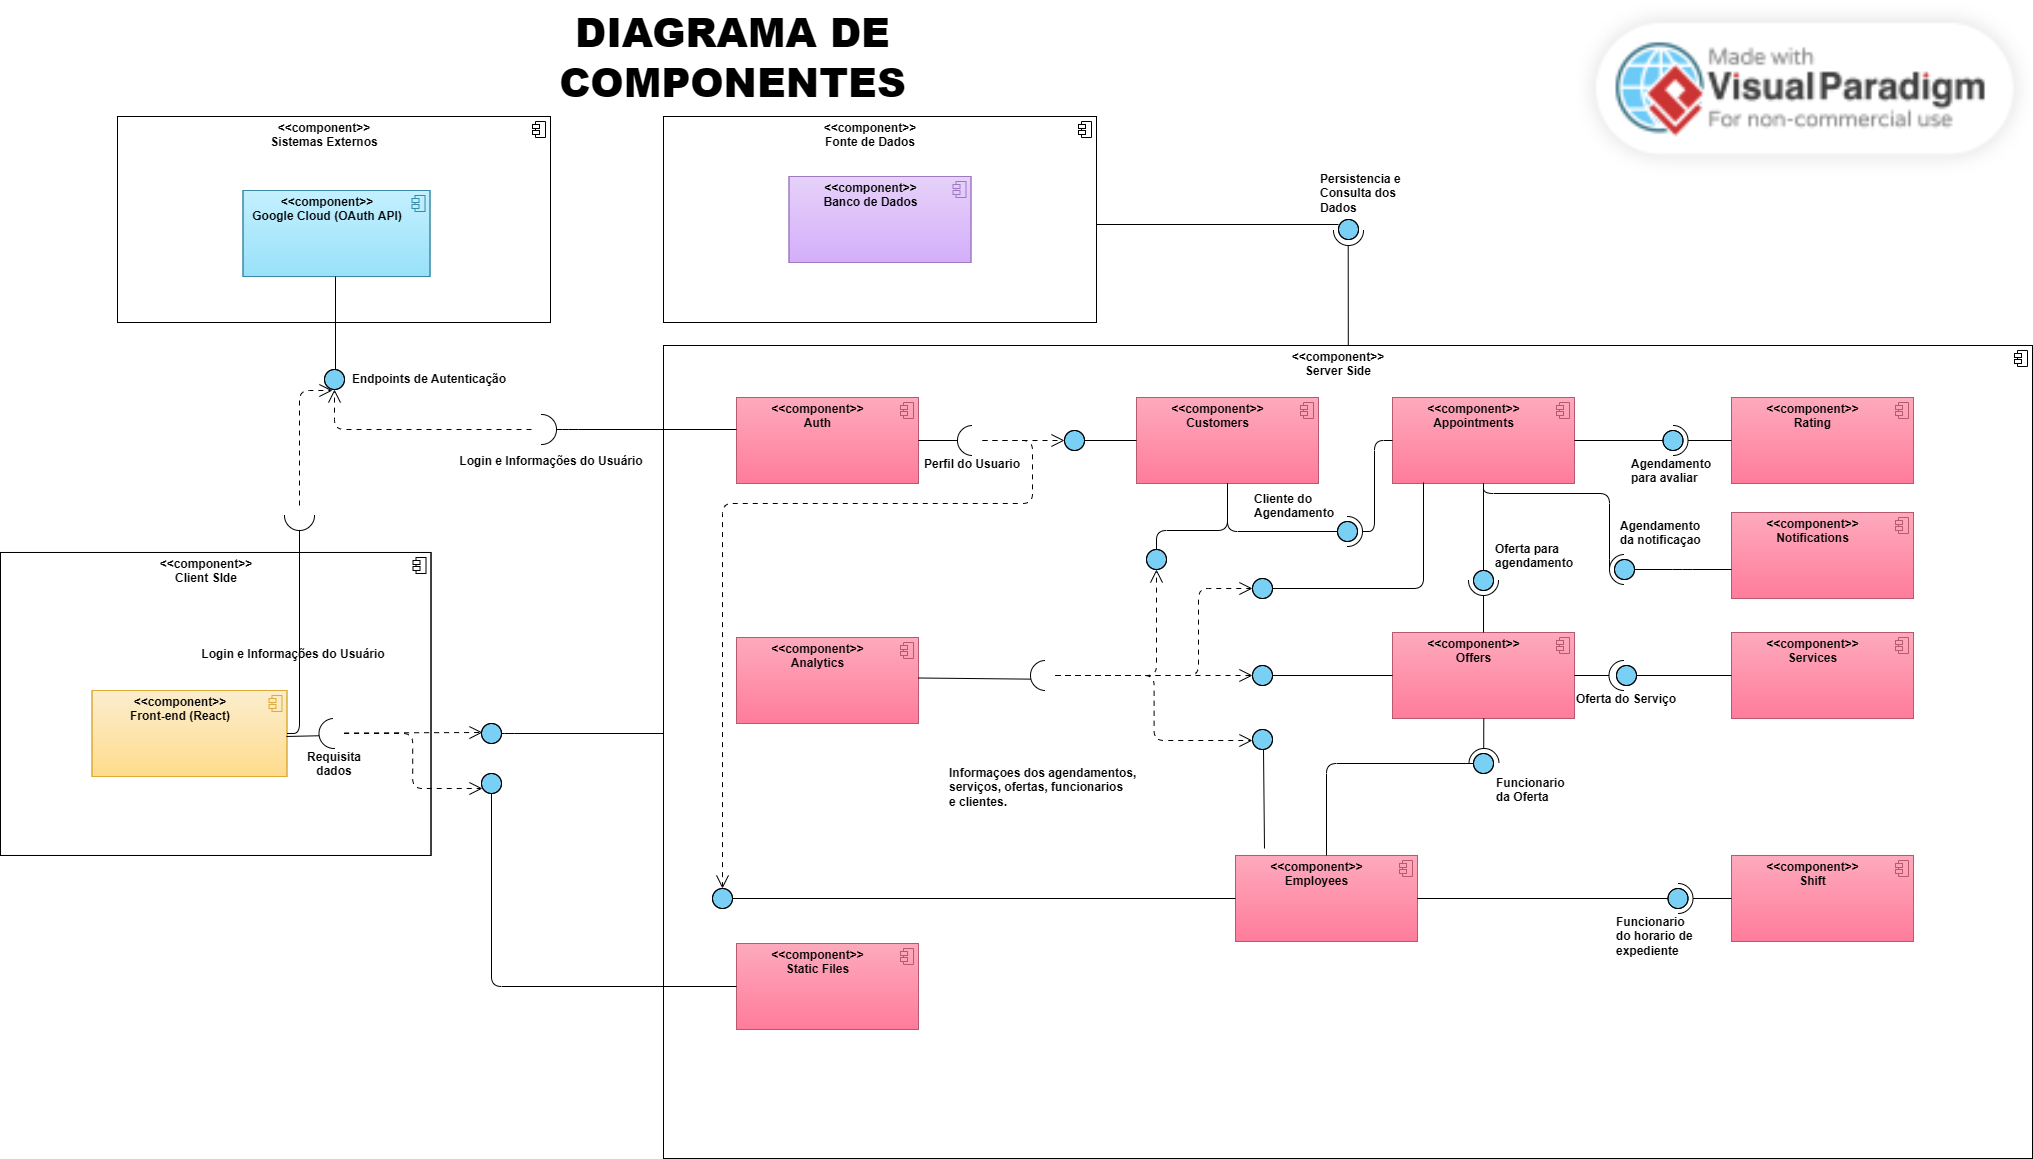
\includegraphics[width=\textwidth]{cap04-desenvolvimento/images/4-3-2-1-diagrama-componentes}
  \label{fig:diagrama-componente}
  \fonte{Produzido pelos autores}
\end{figure}
\FloatBarrier


No diagrama de componentes proposto, a aplicação é composta por diversos módulos que representam funcionalidades distintas e organizadas de forma modular. Esses componentes são responsáveis por encapsular regras de negócio e oferecer interfaces bem definidas para comunicação entre si. A seguir, são descritos os principais módulos do sistema:

\begin{itemize}
  \item \textbf{\emph{Auth}}: Componente responsável pela autenticação de usuários e integração com serviços externos, como o \emph{Google OAuth} \cite{GoogleOAuth}. Garante um processo facilitado de login para os usuários e autenticação no acesso das funcionalidades protegidas da aplicação.

  \item \textbf{\emph{Analytics}}: Responsável por gerar relatórios e fornecer estatísticas baseadas nas informações do sistema. Auxilia principalmente no acompanhamento de desempenho da plataforma por parte dos gerentes do salão.

  \item \textbf{\emph{Appointments}}: Gerencia os agendamentos realizados pelos clientes. Engloba tanto a criação, listagem e atualização dos agendamentos quanto a associação com os serviços ofertados.

  \item \textbf{\emph{Customers}}: Controla os dados relacionados aos clientes da plataforma. Permite o cadastro, consulta e edição de informações do perfil dos usuários.

  \item \textbf{\emph{Professionals}}: Administra os dados dos profissionais que prestam serviços na aplicação, incluindo informações cadastrais, disponibilidade e associação a serviços específicos.

  \item \textbf{\emph{Notifications}}: Responsável por enviar notificações aos usuários, como lembretes, confirmações de agendamento e atualizações importantes. Pode incluir o envio por \emph{e-mail} ou outros canais.

  \item \textbf{\emph{Offers}}: Define a relação entre profissionais e os serviços que eles oferecem. Cada oferta especifica o tempo estimado e o valor cobrado por um profissional para realizar determinado serviço. Esse componente é fundamental para a composição de um agendamento, pois determina quais combinações de profissional e serviço estão disponíveis.

  \item \textbf{\emph{Services}}: Representa os serviços oferecidos pela empresa, armazenando informações descritivas como nome e descrição. Este módulo não define valores ou tempos de execução, pois esses dados são especificados nas ofertas individuais de cada profissional (por meio do módulo \textit{Offers}).

  \item \textbf{\emph{Shift}}: Trata do controle de turnos de trabalho dos profissionais, possibilitando a definição de horários disponíveis para realização dos agendamentos.

  \item \textbf{\emph{Rating}}: Permite que os clientes avaliem os serviços e os profissionais após os atendimentos, promovendo um sistema de \emph{feedback} contínuo.
  
  \item \textbf{\emph{Static Files (Front-end)}}: Componente responsável por servir os arquivos estáticos da interface do usuário, gerados após o processo de \textit{build} do projeto \emph{front-end} (em \emph{React}). Inclui arquivos \gls{html}, \gls{css} e \emph{JavaScript} que são entregues ao navegador do usuário final via servidor \emph{NGINX}.
\end{itemize}

\subsubsection{Diagrama de implantação}

O diagrama de implantação mostra como os componentes do sistema estão distribuídos em termos de infraestrutura~\cite{Booch2005}, seja em servidores físicos ou ambientes virtuais. Ele ajuda a entender onde cada parte da aplicação está rodando, como os serviços se conectam entre si e quais recursos são necessários para que tudo funcione da forma adequada no ambiente de produção.

Esse tipo de representação é especialmente útil para quem for implantar ou manter o sistema, pois facilita a visualização de elementos como servidores, banco de dados, \emph{gateways} de rede, e outras dependências da aplicação. Além disso, o diagrama contribui para o planejamento de permissões, acessos e políticas de segurança que precisam ser configuradas na infraestrutura.

\begin{figure}[htb]
  \centering
  \caption{Diagrama de implantação da aplicação}
  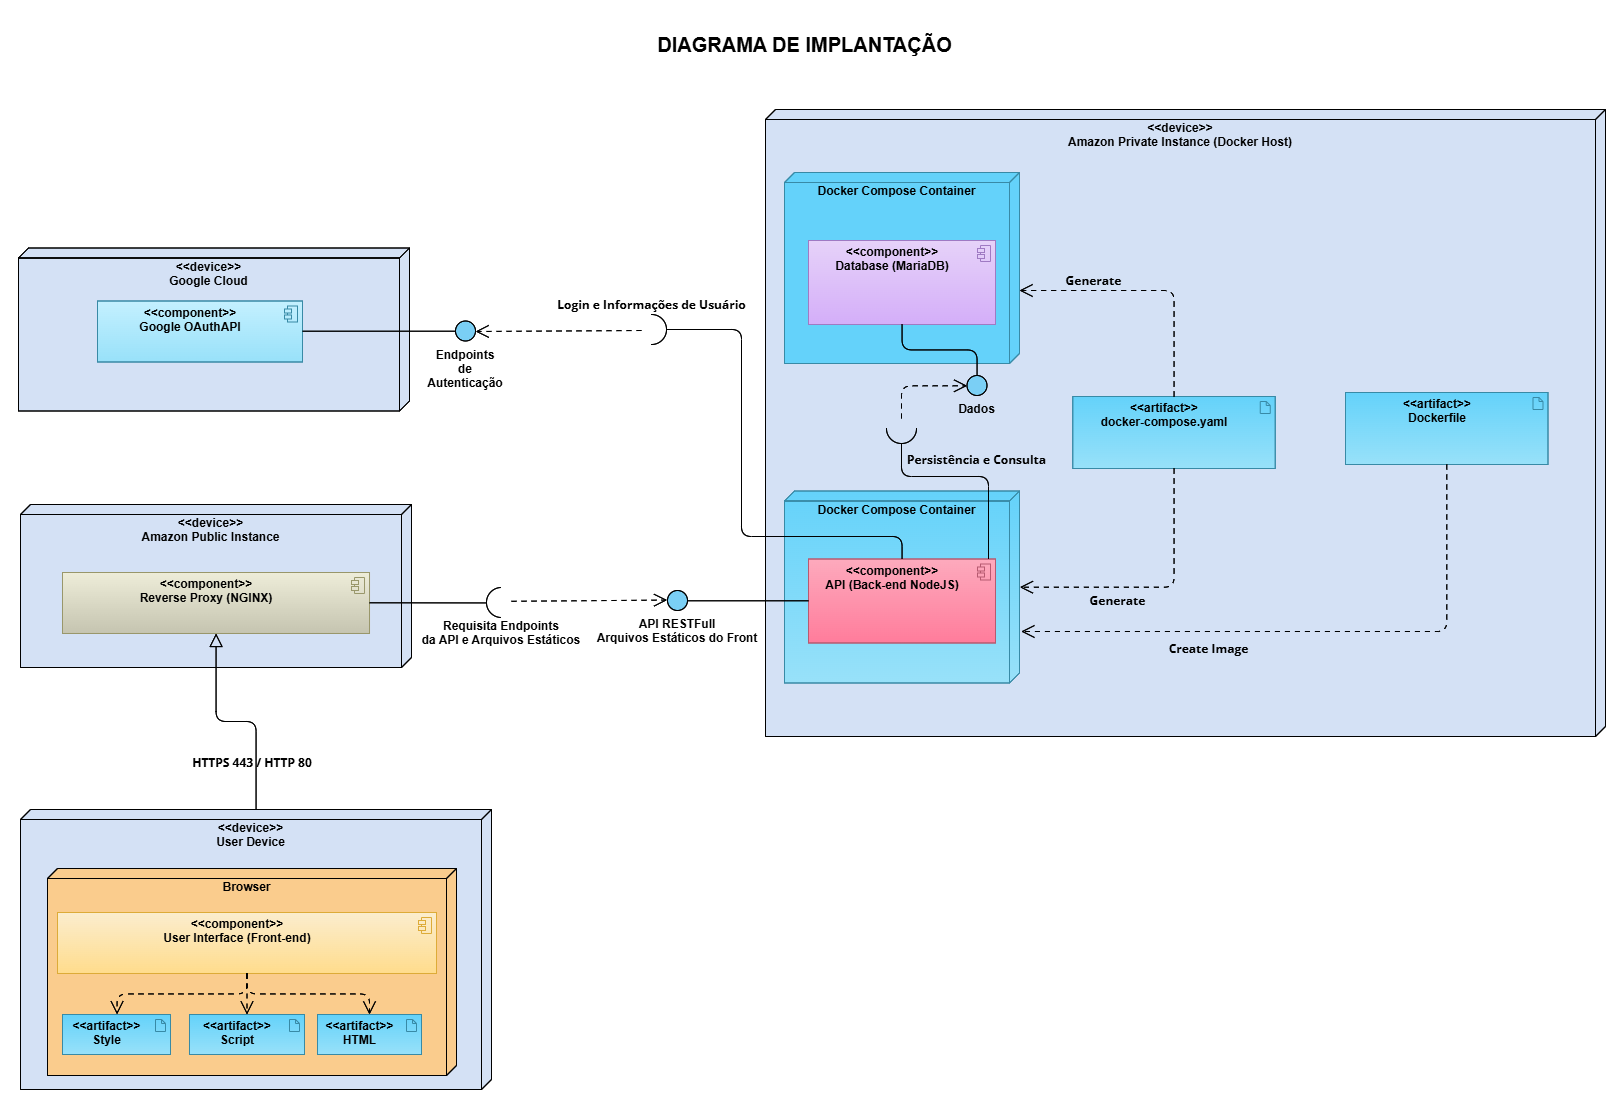
\includegraphics[width=\textwidth]{cap04-desenvolvimento/images/4-3-2-2-diagrama-implantacao}
  \label{fig:diagrama-implantacao}
   \fonte{Produzido pelos autores}
\end{figure}
\FloatBarrier

O diagrama acima é composto pelos seguintes componentes:
\begin{itemize}
  \item \textbf{\textit{User Device:}} No diagrama proposto, por se tratar de uma aplicação \emph{web}, o dispositivo do usuário será responsável por executar a aplicação \textit{client-side}, que interpreta através do navegador os arquivos \gls{css}, \emph{JavaScript} e \gls{html} gerados no empacotamento ou \textit{build} do projeto feito com a biblioteca \emph{React}. Ademais, esse dispositivo é composto por alguns artefatos importantes que são obtidos pelo navegador por meio de uma requisição ao \textit{Proxy Reverso}: \gls{css} (\emph{style)}, \emph{JavaScript} (\emph{script)} e \gls{html}.

  \item \textbf{\textit{Amazon Public Instance (Device):}} A \textit{Amazon Public Instance} é uma instância \gls{ec2} que possui um \gls{ip} público, o que permite que ela seja acessada diretamente pelo usuário ou resolvida por \gls{dns}. Por esse motivo, nela são executados apenas os componentes que devem estar disponíveis publicamente ao cliente final:
    \begin{itemize}
      \item \textit{Componente NGINX}: Serviço que atua como \textit{Proxy Reverso}~\cite{NGINXDocs} para a aplicação que está sendo executada em uma instância privada na arquitetura proposta. Para viabilizar conexões \gls{https}, o \emph{NGINX} utiliza certificados digitais emitidos gratuitamente pelo serviço \emph{Let's Encrypt}, utilizando a ferramenta \emph{Certbot}~\cite{LetsEncryptWithCertbot}, que automatiza todo o processo de emissão e renovação dos certificados. Este serviço é instalado como um \textbf{artefato} adicional no ambiente da instância pública, sendo integrado ao próprio ciclo de configuração e inicialização do \emph{NGINX}.
    \end{itemize}

  \item \textbf{\textit{Amazon Private Instance (Device):}} Por outro lado, a \textit{Amazon Private Instance} é composta por uma instância \gls{ec2} com restrições de rede, o que significa que seu acesso é limitado à rede interna e não possui \gls{ip} público. Nessa instância, componentes da arquitetura que não precisam estar disponíveis de forma pública são o caso de uso perfeito, uma vez que garante maior segurança e isolamento dos aspectos internos da aplicação. Em seu interior, ela é composta pelos seguintes componentes:
    \begin{itemize}
      \item A \textit{\gls{api} (Back-end em NodeJS)}: Principal serviço da aplicação, sendo o responsável por prover os \emph{"endpoints"} que fornecem os dados e arquivos estáticos para o \textit{front-end} através de uma \textit{\gls{api} RestFull}, se comunicando com o banco de dados, um componente que é executado no mesmo dispositivo.
      \item \textit{Banco de Dados (\gls{sgbd} MariaDB)}: Serviço de \gls{sgbd} que provê os dados para o \textit{back-end} da aplicação, o que possibilita a persistência e consulta de forma eficiente. Para garantir a persistência dos dados gerenciados pelo MariaDB, o contêiner utiliza volumes \emph{Docker} montados na instância \gls{ec2} privada. Isso assegura que os dados não sejam perdidos em reinicializações do contêiner.
    \end{itemize}
  Além dos serviços em execução, a instância privada também contém os seguintes artefatos essenciais para o empacotamento e execução dos serviços via contêineres \emph{Docker}~\cite{DockerDocs}:
    \begin{itemize}
      \item \textit{Dockerfile}: Esse artefato descreve as instruções necessárias para criar a imagem \emph{Docker} da aplicação \textit{back-end}, especificando o ambiente base (como a imagem do Node.js), os arquivos a serem copiados, dependências a serem instaladas e os comandos de inicialização da aplicação.

      \item \textit{docker-compose.yaml}: Esse arquivo é utilizado como ferramenta de orquestração para os serviços \emph{Docker}~\cite{DockerComposeDocs} da aplicação. Ele define a configuração dos contêineres da aplicação, como o contêiner da \gls{api} e o do banco de dados, bem como as variáveis de ambiente, volumes, redes e dependências entre os serviços. É a partir deste artefato que os contêineres são gerados e executados de forma integrada.
    \end{itemize}

  \item \textbf{\textit{Google Cloud (Device):}} Localizada na nuvem pública da Google (\textit{Google Cloud}), essa \gls{api} é utilizada pelo \emph{back-end} da aplicação para realizar a autenticação de usuários através do protocolo \emph{OAuth} 2.0 \cite{GoogleOAuth}. Esse processo ocorre quando o usuário opta por fazer \emph{login} com sua conta Google. Nesse cenário, a aplicação redireciona o usuário para a tela de autenticação da Google, e após a confirmação, a \gls{api} recebe um \textit{token} de acesso que é utilizado para obter as informações do usuário autenticado. Esse fluxo garante uma autenticação segura, delegando a responsabilidade da validação de identidade à Google.
\end{itemize}

O fluxo de execução típico da aplicação baseado no diagrama de implantação acima segue os seguintes passos:
\begin{enumerate}
  \item O usuário acessa a aplicação pelo navegador, requisitando os arquivos \gls{html}/\gls{css}/\gls{js} ao servidor \emph{NGINX}.
  \item O \emph{NGINX}, atuando como proxy reverso, redireciona essas requisições para o serviço de \emph{back-end} na instância privada.
  \item A \gls{api} processa a requisição, acessa o banco de dados quando necessário e retorna os dados.
  \item Em caso de autenticação via Google, a \gls{api} redireciona o usuário para o serviço \emph{Google OAuth} \cite{GoogleOAuth}, que retorna um \emph{token} de acesso após o \emph{login}.
  \item Esse \emph{token} é utilizado pela \gls{api} para obter os dados do usuário autenticado e estabelecer uma sessão.
\end{enumerate}

Além da organização dos componentes do diagrama, a arquitetura também prioriza a segurança da comunicação e do acesso. O tráfego entre o navegador do usuário e a instância pública é realizado por meio do protocolo \gls{https}, o que garante a confidencialidade e a integridade dos dados transmitidos. Para isso, foi utilizado o serviço gratuito de certificação digital \emph{Let's Encrypt} em conjunto com a ferramenta \emph{Certbot}, que automatiza a emissão, renovação e instalação dos certificados \gls{tls} no servidor \emph{NGINX}.

Internamente, a comunicação entre o \emph{NGINX} e os serviços da instância privada ocorre seguindo regras específicas de segurança definidas na \gls{vpc}, utilizando mecanismos como \textit{Security Groups} e \textit{Route Tables}. Isso reduz significativamente a superfície de ataque da aplicação e assegura uma camada adicional de proteção para os aspectos internos.

\subsubsection{Diagrama de referência na \gls{aws}}

Com o objetivo de fornecer uma visão mais aprofundada da infraestrutura da aplicação na nuvem, o diagrama apresenta a disposição dos principais componentes implantados na arquitetura da \gls{aws}.

Este diagrama ilustra elementos de infraestrutura fundamentais como sub-redes públicas e privadas, resolução de \gls{dns}, \gls{vpc}, \emph{Bastion Server}, \gls{nat} \emph{Gateway}, \emph{Internet Gateway}, banco de dados, entre outros recursos. A representação facilita a compreensão técnica da topologia de rede e da distribuição dos serviços, evidenciando como a aplicação foi projetada para atender requisitos de segurança, escalabilidade e disponibilidade no ambiente da \gls{aws}. A seguir, descreve-se brevemente cada elemento presente no diagrama.

\begin{figure}[htb]
  \centering
  \caption{Diagrama Geral da Arquitetura}
  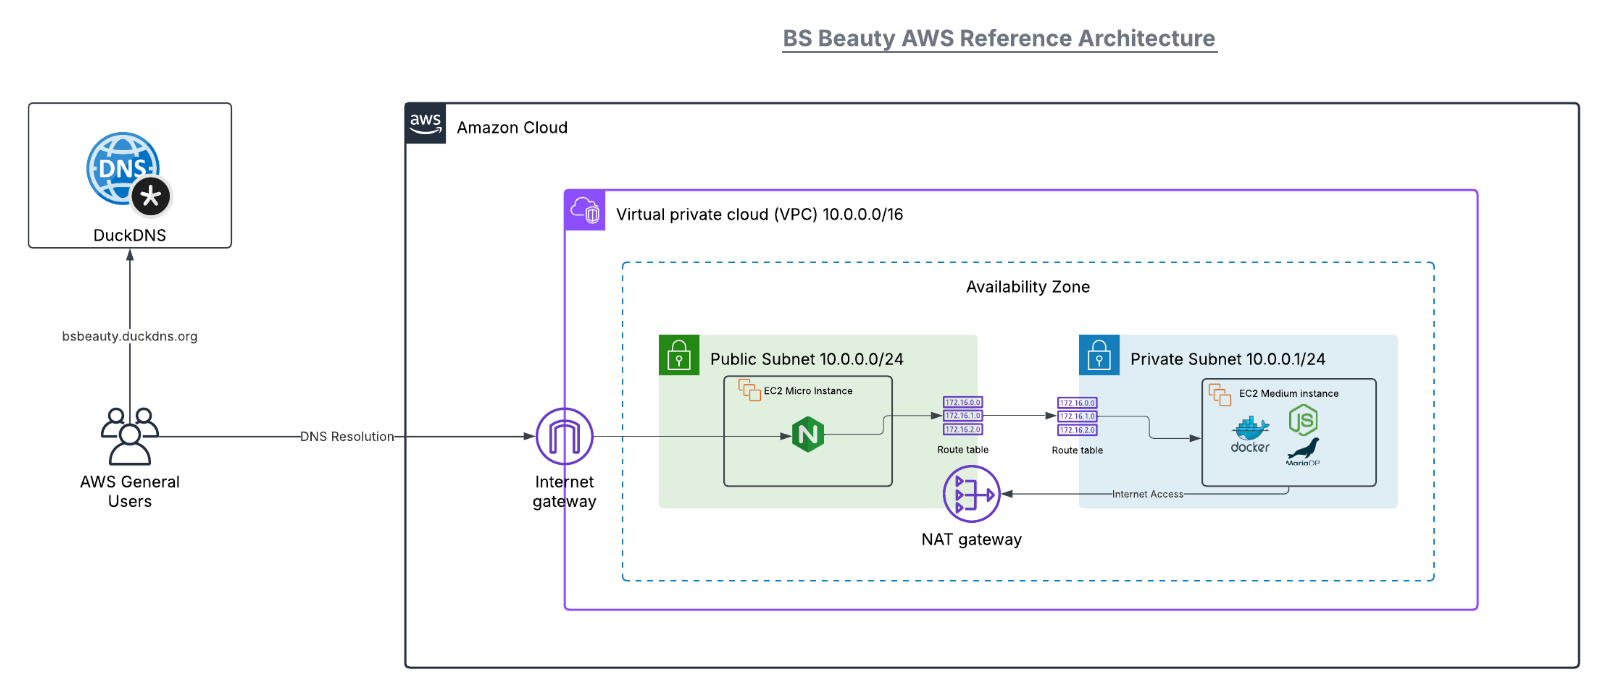
\includegraphics[width=\textwidth]{cap04-desenvolvimento/images/4-3-2-3-diagrama-geral}
  \label{fig:diagrama-geral}
  \fonte{Produzido pelos autores}
\end{figure}
\FloatBarrier

\begin{itemize}
  \item \textbf{\gls{vpc} (Virtual Private Cloud):} A aplicação opera dentro de uma \gls{vpc} personalizada com o bloco \gls{cidr} \texttt{10.0.0.0/16}, que abriga duas sub-redes: uma pública e outra privada, seguindo o princípio de segmentação de rede recomendado pela própria \gls{aws}~\cite{AWSBestPractices}.

  \item \textbf{Sub-rede pública (10.0.0.0/24):} Contém uma instância \gls{ec2} de pequeno porte (\texttt{t2.micro}) que executa o serviço \emph{NGINX}. Esse servidor atua como \emph{proxy} reverso, roteando as requisições provenientes da internet para os serviços internos hospedados em uma sub-rede privada.

  \item \textbf{Sub-rede privada (10.0.0.1/24):} Hospeda uma instância \gls{ec2} de médio porte (\texttt{t2.medium}), na qual são executados os contêineres da aplicação via \emph{Docker Compose}, incluindo o serviço de \emph{back-end} (Node.js) e o banco de dados relacional MariaDB.

  \item \textbf{\gls{nat} \emph{Gateway:}} Permite que os recursos da sub-rede privada (como a instância \gls{ec2} que executa os contêineres) realizem atualizações e acessos à internet de forma segura, sem que sejam diretamente acessíveis externamente.

  \item \textbf{Internet \emph{Gateway:}} Responsável por permitir o tráfego de entrada e saída entre a \gls{vpc} e a internet pública. Está associado à sub-rede pública e \gls{nat} \emph{Gateway}, permitindo que o \emph{NGINX} receba requisições externas e o \gls{nat} receba um \gls{ip}.

  \item \textbf{\emph{DuckDNS:}} Utilizado como serviço de \gls{dns} dinâmico gratuito~\cite{DuckDNSDocs}, permitindo que a aplicação seja acessada por um domínio estável (\texttt{bsbeauty.duckdns.org}), mesmo que o endereço \gls{ip} público da instância \gls{ec2} varie. A resolução de nome é feita de forma transparente para o usuário final, facilitando o acesso à aplicação.

  \item \textbf{Usuários externos (\emph{\gls{aws} General Users):}} Representam os clientes que acessam a aplicação via navegador. O tráfego \gls{http}/\gls{https} chega inicialmente ao serviço \emph{NGINX} na sub-rede pública, que encaminha as requisições para a instância privada onde os serviços da aplicação estão efetivamente em execução.
\end{itemize}

A separação entre sub-rede pública e privada segue boas práticas de segurança e isolamento de ambiente, recomendadas tanto pela documentação oficial da \gls{aws} quanto por autores renomados da área de arquitetura de software em nuvem, como em \cite{AWSBestPractices}. Ao manter os serviços internos em uma sub-rede privada, reduz-se a superfície de ataque da aplicação e melhora a resistência contra acessos não autorizados.

Além disso, a utilização do \emph{DuckDNS} simplifica a exposição da aplicação para o ambiente externo sem a necessidade de configurar manualmente um serviço de \gls{dns} ou pagar por domínios personalizados, o que se alinha aos objetivos de custo deste projeto.
	\section{Tecnologias e Ferramentas} 

\subsection{\emph{Front-End}} 

\subsubsection{\emph{React}} 
O \emph{React} \cite{react} é uma biblioteca \emph{JavaScript} para construção de interfaces de usuário. Atualmente, se coloca como uma das ferramentas mais populares nesse aspecto \cite{state-of-front-end}. Sua utilização se foca na criação de componentes encapsulados, reutilizáveis e que gerenciam seus próprios estados.

\begin{figure}[htb]
	\centering
	
\includegraphics[width=6cm]{cap04-desenvolvimento/images/4-4-1-1-react}
	\caption{Logo do \emph{React}}
	\label{fig:logo_react}
	\fonte{\cite{react-logo}}
\end{figure}

\subsubsection{\emph{TailwindCSS}} 
\emph{Framework} de \gls{css} utilitário que permite a criação rápida de \emph{layouts} e estilizações diretamente nas classes \gls{html}. Parte da premissa do desenvolvedor não deixar o arquivo \gls{html} para estilizar a página com \gls{css}, embutindo as duas tecnologias em um único arquivo e também removendo código \gls{css} inútil, diminuindo o tamanho do arquivo final enviado ao usuário final \cite{tailwind}.

\begin{figure}[htb]
	\centering
	
\includegraphics[width=6cm]{cap04-desenvolvimento/images/4-4-1-2-tailwindcss-logotype.svg}
	\caption{Logo do \emph{Tailwind}}
	\label{fig:logo_tailwind}
	\fonte{\cite{tailwind-logo}}
\end{figure}

\subsubsection{\emph{Redux} e \emph{RTK Query}} 
Biblioteca que facilita o gerenciamento de estados no \emph{React} e outras bibliotecas de \emph{interface }\cite{redux}. Já o \emph{RTK Query} oferece funcionalidades de cache e requisições assíncronas de forma otimizada \cite{rtk-query}. Ele facilita a criação de código para requisição de dados, evitando sua escrita manual, que torna-se muito repetitiva no desenvolvimento de aplicações. 

\subsection{\emph{Back-End}} 

\subsubsection{\emph{NodeJS}} 
Ambiente de execução \emph{JavaScript} no lado do servidor, baseado no motor V8 do navegador \emph{Chrome}. É ideal para a construção de aplicações escaláveis e que funcionem em tempo real \cite{node}. O fato de funcionar independentemente do navegador torna-o performático e atraente para os desenvolvedores.

\subsubsection{\emph{Express}} 
\emph{Framework} de roteamento minimalista para Node.js que torna a criação de \gls{api}s e rotas \gls{http} simples e eficiente. Ele possui uma enxuta gama de ferramentas e recursos, que providenciam uma forma facilitada para criação de aplicações sem comprometer a já aclamada performance do Node \cite{express}, no entanto, suas funcionalidades ainda podem ser ampliadas pelos módulos de \emph{middleware}.

\subsection{Infraestrutura} 

\subsubsection{\emph{Docker}}
Plataforma aberta de contêineres que permite empacotar aplicações e suas dependências de forma isolada e reprodutível. Essa divisão entre infraestrutura e aplicação culmina na entrega mais veloz de \emph{software}, e o encapsulamento de aplicações elimina os problemas que surgem por diferenças em relação a \emph{hardware} ou sistema operacional. Um contêiner \emph{Docker} funciona para qualquer pessoa da mesma forma \cite{docker}.

\subsubsection{\emph{Amazon Web Services} (\gls{aws})} 
É uma plataforma que provê computação em nuvem. Esses serviços são utilizados para hospedagem, armazenamento, orquestração de infraestrutura e muito mais \cite{aws}.

\subsubsection{Banco de Dados MariaDB}
Notável e popular Sistema de gerenciamento de banco de dados relacional \emph{Open Source} usado para armazenamento persistente e estruturado de dados. Trata-se de um \emph{fork} do \emph{MySQL}, feito pelos seus desenvolvedores originais após a aquisição deste último pela \emph{Oracle} \cite{mariadb}.

\subsection{Qualidade de Software e Testes} 

\subsubsection{\emph{SonarQube}} 
Ferramenta para análise contínua da qualidade do código, identificando problemas como \emph{bugs}, vulnerabilidades e \emph{code smells} \cite{sonarqube}.

\subsubsection{\emph{Vitest}}
\emph{Framework} moderno de testes para aplicações \emph{JavaScript} e \emph{TypeScript}, com integração nativa ao ecossistema do Vite \cite{vitest-2025}.

	\section{Testes e Manutenibilidade}
Nessa seção do capítulo, apresenta-se os mecanismos e ferramentas adotados para garantir a qualidade de software do projeto ao longo do desenvolvimento.
Será abordado o plano de testes, assim como cada teste que está incluso. Além disso, assuntos como infraestrutura de testes e convenções de código (coding convention)
serão detalhados, evidenciando práticas que promovem a manutenibilidade, padronização e confiabilidade do sistema ao longo de sua evolução.

\subsection{Plano de Testes}
O plano de testes define a estratégia adotada para garantir a qualidade e confiabilidade da aplicação. 
Ele inclui os tipos de testes aplicados, as ferramentas utilizadas, o escopo das validações, e os critérios de sucesso e falha.

Tendo em vista que a arquitetura do back-end é constituída por \textit{controllers}, \textit{services} e \textit{repositories} usando o framework \textbf{Express}, 
é necessário garantir um ótimo funcionamento da comunicação entre essas camadas. Portanto, conforme os recursos da RESTful API
são desenvolvidos (agendamentos, serviços de beleza, clientes, funcionários, etc) com as respectivas camadas que foram comentadas,
urge-se a demanda de serem testadas em paralelo, cobrindo os cenários possíveis cenários de sucesso/falha. 

Pretende-se atingir, no mínimo, 80\% de cobertura nos testes unitários e integrados aplicados 
sobre as camadas de \textit{controllers} e \textit{services} da API. 
Essa métrica será obtida por meio de ferramentas integradas ao ambiente de testes, como o \textbf{Vitest} com suporte a geração de relatórios de cobertura. Embora a cobertura de testes não garanta por si só a ausência de falhas, ela serve como um forte indicador de que a maior parte da lógica de negócio está sendo exercitada e validada durante a execução dos testes. Essa prática contribui diretamente para a robustez do sistema 
e facilita a detecção precoce de regressões ao longo do desenvolvimento.

O mesmo propósito de cobertura de testes é válido para o front-end desenvolvido em \textbf{React}. Como essa tecnologia adota um princípio de componentização de elementos da interface,
é interessante que as páginas com cenários lógicos mais críticos (como as telas de agendamento) sejam validadas de forma precisa.
Garantindo que os elementos da interface estejam atendendo o comportamento esperado.

Quanto à cobertura de testes do front-end, é tido como propósito, realizar uma cobertura de testes automatizados que envolva todos os processos que foram mapeados no escopo do projeto.

Os arquivos contendo as classes/funções de testes devem estar localizados em diretórios específicos 
de testes, adotando uma nomenclatura compreensível como 
\texttt{analytics.\allowbreak controller.\allowbreak spec.\allowbreak unit.ts} (referenciando um teste unitário) e 
\texttt{analytics.\allowbreak controller.\allowbreak spec.\allowbreak integration.ts} (referenciando um teste integrado).

\subsection{Infraestrutura de Testes}

A infraestrutura de testes do projeto está fortemente integrada ao processo de integração contínua (CI) e entrega contínua (CD),
utilizando a ferramenta \textbf{GitHub Actions}. Essa integração visa garantir que o código entregue atenda a padrões mínimos de qualidade e estabilidade 
em todas as etapas do desenvolvimento.  A cada push ou pull request, fluxos automatizados são executados para validar o código por meio de testes automatizados, 
análise estática, e verificação de cobertura. Esse processo assegura que apenas alterações estáveis e em conformidade com os 
padrões de qualidade sejam incorporadas à base de código principal, promovendo entregas seguras e contínuas ao longo do ciclo de desenvolvimento.

\subsection{Análise Estáticas}
A análise estática de código é realizada utilizando a ferramenta \textbf{SonarQube}, 
que permite detectar problemas de qualidade, como vulnerabilidades, bugs e código duplicado, sem a necessidade de executar a aplicação. 
Essa etapa ajuda a manter o código limpo, seguro e sustentável ao longo do tempo.

\subsection{Testes Automatizados}
A automação de testes tem como objetivo aumentar a confiabilidade do software e permitir validações rápidas e constantes. O projeto conta com:

\begin{itemize}
  \item \textbf{Testes unitários:} Validam o comportamento de funções e componentes isolados. \textbf{Vitest}.
  \item \textbf{Testes integrados:} Verificam a interação entre módulos e componentes da aplicação, também utilizando o \textbf{Vitest}.
%  \item \textbf{Testes de interface:} Serão aplicados, se necessário, nas páginas de maior relevância funcional da aplicação. Ferramentas como \textbf{Cypress} poderão ser utilizadas.
\end{itemize}

\subsection{Logs}
\subsection{Code Convention}
Para garantir a legibilidade e padronização do código, são adotadas convenções definidas com base em boas práticas da comunidade JavaScript/TypeScript.
Essas diretrizes ajudam a manter o código uniforme entre os diferentes desenvolvedores do time, reduzindo ambiguidades e facilitando o entendimento do sistema como um todo.


As principais práticas adotadas incluem:

\begin{itemize}
  \item \textbf{Ferramentas de Linting e Formatação:}
  \begin{itemize}
    \item Utilização do \textbf{ESLint} para garantir padrões de estilo e detectar possíveis erros ou práticas inadequadas de codificação.
    \item Uso do \textbf{Prettier} para formatação automática do código, assegurando que todos os arquivos mantenham a mesma estrutura visual (espaçamento, quebras de linha, indentação, etc).
  \end{itemize}

  \item \textbf{Padrões de Nomenclatura:}
  \begin{itemize}
    \item Uso de \texttt{camelCase} para variáveis e funções.
    \item Uso de \texttt{PascalCase} para componentes e classes.
    \item Uso de \texttt{UPPER\_SNAKE\_CASE} para constantes globais.
  \end{itemize}

  \item \textbf{Organização do Código:}
  \begin{itemize}
    \item Estrutura modular com separação clara entre camadas (controllers, services, repositories).
    \item Agrupamento de arquivos por domínio funcional.
  \end{itemize}

  \item \textbf{Boas Práticas:}
  \begin{itemize}
    \item Escrita de código limpo e legível, evitando duplicações.
    \item Utilização de comentários apenas quando necessário, priorizando nomes autoexplicativos.
    \item Aplicação do princípio DRY (Don't Repeat Yourself).
  \end{itemize}

  \item \textbf{Revisões e Padronização em Equipe:}
  \begin{itemize}
    \item Adoção de pull requests com as devidas descrições das funcionalidades desenvolvidas.
    \item Documentação e comunicação clara de decisões técnicas relevantes.
  \end{itemize}
\end{itemize}
% \subsection{Testes de Performance}
% \subsection{Testes de Componente}
% \subsection{Testes Funcionais}
% \subsection{Testes não Funcionais}
% \subsection{Testes de Carga}
% \subsection{Testes de Configuração}
	\section{Segurança, Privacidade e Legislação}
Atualmente, há uma crescente no número de usuários utilizando dispositivos conectados a \textit{Internet}, o que, por um lado mostra que essa tecnologia tão importante está sendo difundida a todas as camadas sociais, mas por outro, gera preocupação quanto as implicações do uso inadvertido das redes.
Nesse contexto, tornou-se comum pessoas mal intencionadas que usam da ignorância de alguns para cometer ataques digitais, prejudicando ou tomando vantagem de pessoas, grupos ou organizações. A afirmativa anterior é confirmada por um gráfico (Figura \ref{fig:cibercrimes}) elaborado pela \emph{Surfshark} \cite{Surfshark}, empresa provedora de serviços de \gls{vpn}, que analisa o crescimento anual de custos em cibersegurança. 
\begin{figure}[h]
	\centering
	\caption{Crescimento anual de custos com cibercrime}
	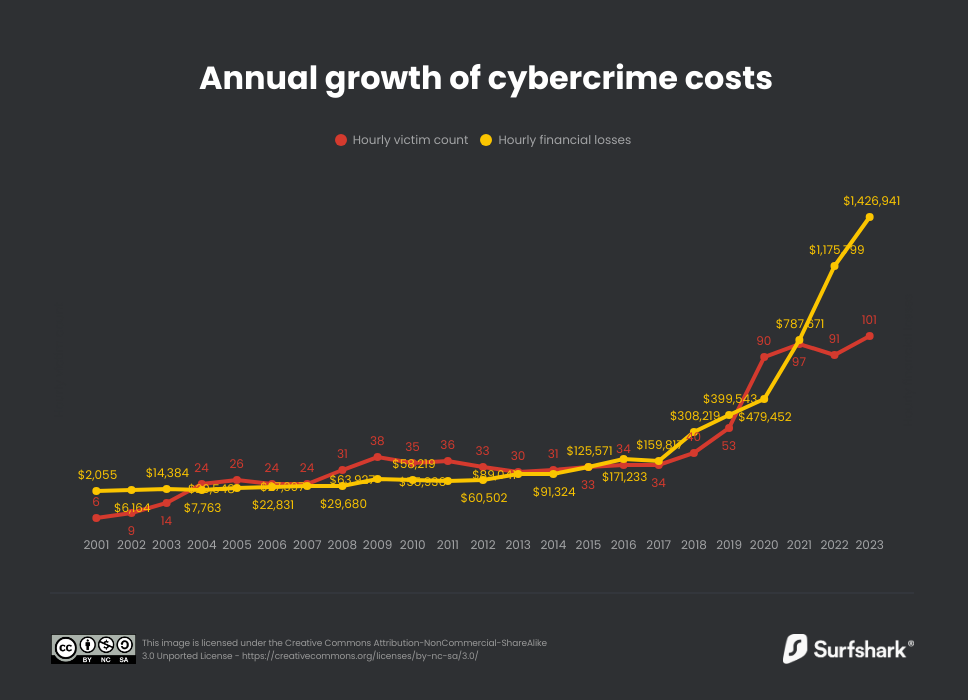
\includegraphics[width=1\textwidth]{cap04-desenvolvimento/images/4-6-annual-growth-of-cybercrime-costs.png}
	\fonte{\cite{Surfshark}}
	\label{fig:cibercrimes}
\end{figure}

Por isso surgiram leis e normas que regularizam como os dados devem ser tratados e também tecnologias que auxiliam a proteger os dois lados da comunicação: os clientes, que desejam ter seus dados protegidos, e das organizações, que precisam se certificar da identidade do usuário.
Isto posto, serão abordadas as técnicas e metodologias adotadas a fim de garantir que o software desenvolvido atenda as demandas da legislação e promova segurança e privacidade a seus utilizadores.

\subsection{Critérios de Segurança e Privacidade}
Na aplicação desenvolvida, foram definidas formas de manter a segurança de todas as partes envolvidas. Foi implementado um método de cadastro e \textit{login} facilitado com geração de \textit{tokens} e também uma infraestrutura de rede que protege o dispositivo que armazena o banco de dados da aplicação.

\subsubsection{Cadastro e \emph{Login} com Conta Google}
Um dos requisitos da entidade parceira, era o desenvolvimento de um sistema de cadastro e \emph{login} facilitados, haja vista que muitos dos clientes tinham dificuldade em acessar a aplicação anterior por constantemente esquecerem sua credenciais (\emph{e-mail} e senha).
Considerando essa dificuldade, foi implementado um sistema de registro e \emph{login} utilizando a \gls{api} de autenticação \emph{OAuth} da Google, pelo fato da maioria dos dispositivos no Brasil apresentarem sistema operacional Android, conforme destaca uma pesquisa \cite{app-my-site}, que geralmente requerem uma conta Google para seu funcionamento. E mesmo indivíduos com aparelhos de outro sistema operacional, comumente possuem contas Google para usufruir de seus serviços.
Assim sendo, a responsabilidade de identificar os usuários da aplicação foi terceirizada para a Google, e quando estes se cadastram, devem aceitar suas políticas e termos de usuário que definem extensamente como os dados são processados, tratados e protegidos.

\subsubsection{Infraestrutura de Rede}
Os dispositivos (máquinas virtuais) que sustentam a aplicação estão hospedados na \gls{aws}, logo sendo de sua inteira responsabilidade protegê-los fisicamente, como diz seu Modelo de Responsabilidade Compartilhada \cite{aws-shared-responsibilities}, porém no que tange a software e redes, cabe ao time de desenvolvimento proteger.
Para evitar acessos indevidos aos sistema interno, criaram-se duas instâncias \gls{ec2}, uma delas sendo pública e outra privada. Como já explicado, a instância privada não possui \gls{ip} público, portanto só é possível acessá-la pela rede interna dentro da infraestrutura de rede criada, delimitando uma camada a mais de segurança.
O acesso a essa instância é feito pela instância pública por meio do protocolo \gls{ssh}, que possui seus próprios métodos de segurança com esquema de chaves de acesso.

\subsubsection{Controle de Acesso Baseado em Papéis}
Outra medida de segurança, dessa vez mais relacionada a estrutura do software em si, é o controle de acesso baseado em \textit{roles}, traduzido geralmente como papéis.
Na aplicação desenvolvida existem diversas páginas disponíveis, sendo cada uma delas destinada a um tipo de usuário (papel), como gerente, funcionários ou clientes. Assim, faz-se necessário uma maneira de bloquear e liberar o acesso a esses recursos conforme o papel do usuário atual, evitando que clientes do salão tenham acesso a páginas de relatório por exemplo.
O controle de acesso foi implementado por meio do mapeamento dos papéis e permissões dentro da aplicação. Consequentemente, toda vez que uma página é requisitada, faz-se uma verificação do papel do usuário atual, que recebe ou não permissão para acessá-la.
Dessa forma os recursos são disponibilizados de forma consoante ao usuário. Resolvendo o problema de acessos indevidos a partes do sistema e também tornando a experiência do usuário coerente.

\subsection{Observância à Legislação}
No Brasil a legislação que define como os dados devem ser manipulados digitalmente é a Lei Geral de Proteção de Dados, conhecida pelo seu acrônimo \gls{lgpd} \cite{lgpd}. De acordo com a \gls{lgpd}, os dados que coletamos não se enquadram como dados sensíveis, mas apenas como dados pessoais, portanto a aplicação se isenta de muitas restrições legislativas.

Para utilização dos dados pessoais coletados, foi elaborada uma política de usuário que deve ser aceita antes que se conclua o cadastro na plataforma, provendo informações sobre quais dados estão sendo coletados, para qual finalidade e como são tratados.  Esses dados não são utilizados de forma a prejudicar o usuário, excluindo ou tratando-o de maneira diferente por motivos pessoais, políticos ou étnicos. 

Ademais, o usuário pode visualizar e alterar esses dados a qualquer momento dentro da aplicação sem quaisquer tipo de restrição e como já discutido, diversos mecanismos de segurança foram implementados e empresas consolidadas no ramo de tecnologia são responsáveis pelas questões de infraestrutura física e autenticação, garantindo a integridade, confidencialidade e disponibilidade dos recursos.
	\section{Modelo de Banco de Dados}
Para o desenvolvimento da aplicação foram elaborados previamente modelos de representação do banco de dados. Tais modelos auxiliam a ter uma visão da aplicação antes que seja de fato desenvolvida.
\subsection{Modelo Entidade Relacionamento - MER}
O \gls{mer} explica muito sobre a aplicação e já aponta algumas regras de negócio.
Nele foram definidas as seguintes entidades e relacionamentos:
\begin{itemize}
	\item \emph{CUSTOMER}: Entidade que representa um cliente.
	\begin{itemize}
		\item \textbf{\textit{refers:}} um cliente (\emph{CUSTOMER}) pode ou não indicar (\textit{refers}) outros clientes e um cliente é indicado por nenhum ou um único cliente.
		\item \textbf{\textit{makes:}} um cliente faz (\emph{makes}) ou não agendamentos (\emph{APPOINTMENT}).
	\end{itemize}
	\item \emph{APPOINTMENT}: Entidade que representa um agendamento.
	\begin{itemize}
		\item \textbf{\textit{makes}}: um agendamento (\emph{APPOINTMENT}) é feito (\textit{makes}) por um cliente (\emph{CUSTOMER}). 
		\item \textbf{\textit{has}}: um agendamento (\emph{APPOINTMENT}) tem (\textit{has}) ou não uma avaliação (\emph{RATING}).
		\item \textbf{\textit{sends}}: um agendamento (\emph{APPOINTMENT}) envia (\textit{sends}) ao menos uma notificação (\emph{NOTIFICATION}).
		\item \textbf{\textit{includes}}: um agendamento (\emph{APPOINTMENT}) inclui (\textit{includes}) uma oferta (\emph{OFFER}).
	\end{itemize}
	\item \emph{RATING}: Entidade que representa a avaliação de um agendamento.
	\begin{itemize}
		\item \textbf{\textit{has:}} uma avaliação (\emph{RATING}) é tida (\textit{has}) por um agendamento (\emph{APPOINTMENT}).
	\end{itemize}
	\item \emph{NOTIFICATION}: Entidade que representa uma notificação.
	\begin{itemize}
		\item \textbf{\textit{sends:}} uma notificação (\emph{NOTIFICATION}) é enviada por (\textit{sends}) um agendamento (\emph{APPOINTMENT}).
	\end{itemize}
	\item \emph{OFFER}: Entidade associativa que representa a oferta (\textit{offers}) de um serviço (\emph{SERVICE}) por um funcionário (\emph{EMPLOYEE}).
	\begin{itemize}
		\item \textbf{\textit{includes}}: uma oferta (\emph{OFFER}) pode ou não ser incluida (\textit{includes}) em muitos agendamentos (\emph{APPOINTMENT}). 
	\end{itemize}
	\item \emph{EMPLOYEE}: Entidade que representa um funcionário.
	\begin{itemize}
		\item \textbf{\textit{offers}}: um funcionário (\emph{EMPLOYEE}) oferece (\textit{offers}) ou não muitos serviços (\emph{SERVICE}).
		\item \textbf{\textit{has}}: um funcionário (\emph{EMPLOYEE}) tem (\textit{has}) ou não muitos turnos (\emph{SHIFT}).
		\item \textbf{\textit{has}}: um funcionário (\emph{EMPLOYEE}) tem (\textit{has}) ao menos um papel (\emph{ROLE}).
	\end{itemize}
	\item \emph{SERVICE}: Entidade que representa um serviço no salão de beleza.
	\begin{itemize}
		\item \textbf{\textit{offers}}: um serviço (\emph{SERVICE}) é oferecido (\textit{offers}) ou não por muitos funcionários (\emph{EMPLOYEE}).
	\end{itemize}
	\item \emph{SHIFT}: Entidade que representa os turnos de trabalho de um funcionário.
	\begin{itemize}
		\item \textbf{\textit{has}}: um turno (\emph{SHIFT}) é tido (\textit{has}) por um funcionário (\emph{EMPLOYEE}).
	\end{itemize}
	\item \emph{ROLE}: Entidade que representa os papéis que um funcionário possui na plataforma.
	\begin{itemize}
		\item \textbf{\textit{has}}: um papel (\emph{ROLE}) é tido ou não (\textit{has}) por muitos funcionários (\emph{EMPLOYEE}).
		\item \textbf{\textit{has}}: um papel (\emph{ROLE}) tem (\textit{has}) ao menos uma permissão (\emph{PERMISSIONS}).
	\end{itemize}
	\item \emph{EMPLOYE\_ROLE}: Entidade associativa auxiliar para \emph{EMPLOYEE} e \emph{ROLE}.
	\item \emph{PERMISSIONS}: Entidade que representa as permissões que cada papel provê.
	\begin{itemize}
		\item \textbf{\textit{has}}: uma permissão (\emph{PERMISSIONS}) é tida (\textit{has}) ou não por muitos papeis (\emph{ROLE}).
\end{itemize}
	\item \emph{ROLE\_PERMISSION}: Entidade associativa auxiliar para \emph{ROLE} e \emph{PERMISSIONS}.
\end{itemize}
\begin{figure}[h!tbp]
	\centering
	\caption{MER}
	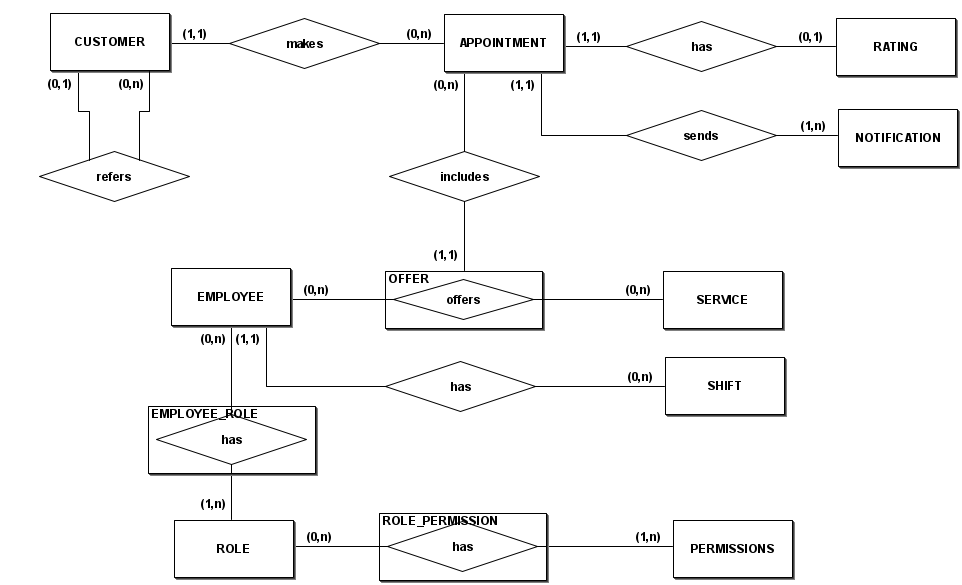
\includegraphics[width=1\textwidth]{cap04-desenvolvimento/images/4-7-1-modelo-entidade-relacionamento.png}
	\fonte{Produzido pelos autores}
	\label{fig:mer}
\end{figure}
\subsection{Diagrama Entidade Relacionamento - DER}
Após a elaboração do \gls{mer} conforme o entendimento dos requisitos e necessidades da entidade parceira, foi produzido um \gls{der}, a partir do \gls{mer}, que contém a listagem de todos os atributos das entidades modeladas, apresentando seus nomes, o tipo de dado e sua possível categorização como chave primária (identificadora) ou estrangeira.
\begin{figure}[h!tbp]
	\centering
	\caption{DER}
	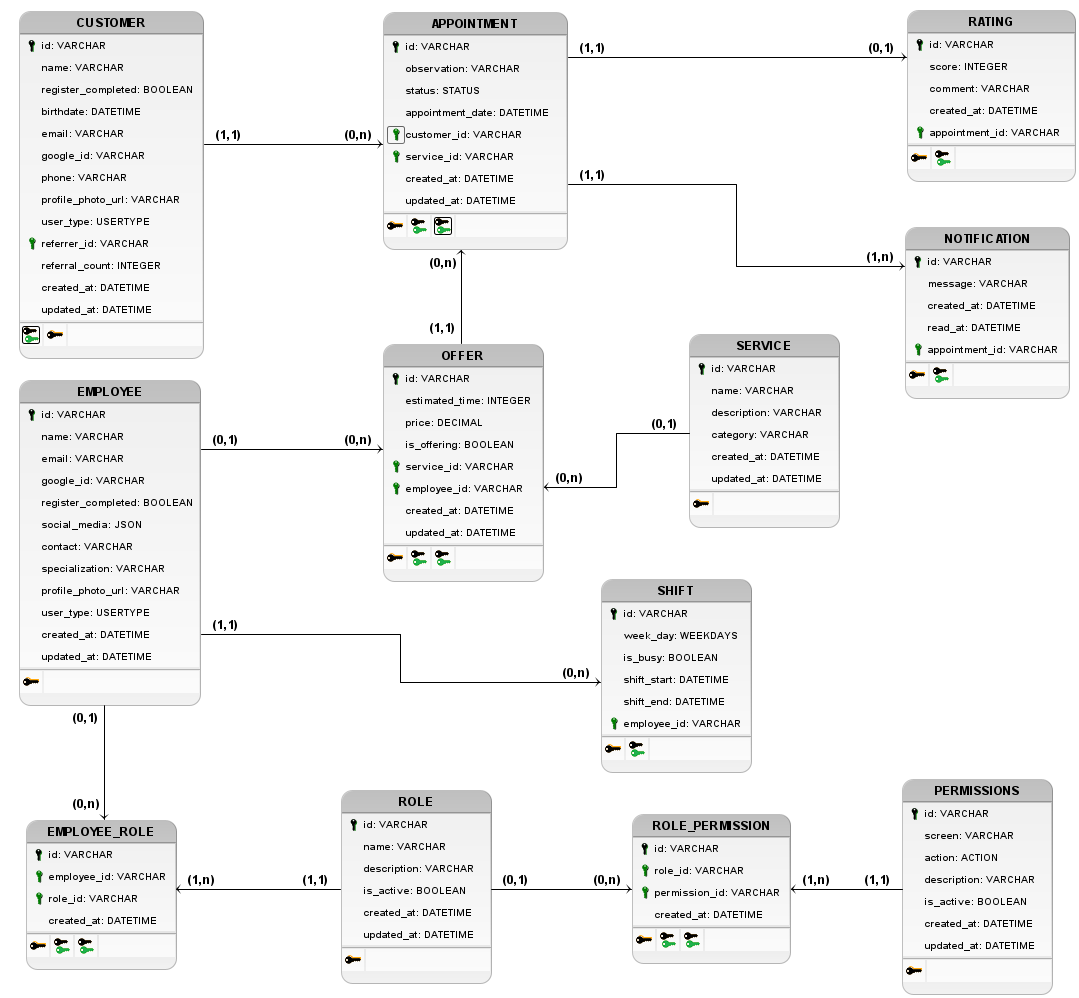
\includegraphics[width=1\textwidth]{cap04-desenvolvimento/images/4-7-2-diagrama-entidade-relacionamento.png}
	\fonte{Produzido pelos autores}
	\label{fig:der}
\end{figure}
\subsection{Dicionário de Dados}
Pensando no modelo físico de banco de dados, também foi elaborado um dicionário de dados referente ao sistema que se enquadra como uma poderosa ferramenta de documentação. Com esse instrumento, qualquer pessoa pode entender como foi pensado os atributos do sistema, como são armazenados e qual seria a finalidade de cada um.
O dicionário descreve:
\begin{itemize}
	\item \textbf{\gls{pk}/\gls{fk}:} Se um atributo é chave primária ou estrangeira.
	\item \textbf{Nome do Campo:} Qual o nome do atributo.
	\item \textbf{Tipo:} Qual o tipo de dado do atributo, como \textit{INT} para valores numéricos inteiros.
	\item \textbf{Descrição:} A descrição do atributo, explicando o que representa na prática.
	\item \textbf{\textit{Null:}} Se o campo pode ser nulo, ou seja, não ter valor atribuído.
	\item \textbf{Tamanho:} O tamanho do atributo, como quantidade de caracteres (\textit{bytes}).
	\item \textbf{Valores permitidos:} Quais os valores permitidos para atributos. Alguns campos utilizam enumerações, por exemplo, que possuem valores definidos previamente.
	\item \textbf{Observações:} Algumas especificidades, como valores padrão, ou de onde uma \gls{fk} foi tomada.
\end{itemize}
Abaixo se encontra um \textit{QR Code} que leva à planilha onde foi elaborado o dicionário de dados desta aplicação.
\begin{figure}[h]
	\centering
	\caption{\emph{QR Code} do Dicionário de Dados}
	\label{fig:qrcode-dicionario-de-dados}
	\scalebox{1.5}{\qrcode{https://docs.google.com/spreadsheets/d/17kJ2aQqjXM-HIXZLWUs257oe_hur0jlTakR0s9KdBrE}}
	\fonte{Produzido pelos autores}
\end{figure}






	
	%---

	%---   
	\section{Cronograma}
	pensar no projeto todo, não só MVP
	\subsection{Análise da Duração do Projeto}
	considerar o gerenciamento ágil
	
	% ----------------------------------------------------------
	
	\chapter{Viabilidade Financeira}
	
	mesmo usando uma hospedagem gratis (AWS), precisamos pesquisar uma paga para colocar na tabela de custos
	
	\section{Custos}
	
	\section{Receitas}
	\section{Cenário realista}
	\section{Cenário Otimista}
	\section{Cenário Pessimista}
	% ---------------------------------------------------------------
	
	\chapter{Considerações Finais}
	\section{Dificuldades, escolhas e Descartes}
	\cite{ibge1993}
	% ----------------------------------------------------------
	
	ver documento "abntex2-modelo-include-comandos" para dicas e tutoriais de como fazer tabelas, graficos, quadros, inserir imagens e documentos externos etc aqui. 
	% ---
	
	%Página de referencias
	\renewcommand{\bibname}{Referências Bibliográficas} %renomeia o título da página de referencias
	\bibliography{referencias-bibliograficas}
	\bibliographystyle{abntex2-alf}
	\bibliographystyle{abntex2-num}
	
	
	% ----------------------------------------------------------
	% Glossário
	% ----------------------------------------------------------
	%
	% Consulte o manual da classe abntex2 para orientações sobre o glossário.
	%
	%\glossary
	
	% ----------------------------------------------------------
	% Apêndices
	% ----------------------------------------------------------
	
	% ---
	% Inicia os apêndices
	% ---
	\begin{apendicesenv}
		
		% Imprime uma página indicando o início dos apêndices
		\partapendices
		
		% ----------------------------------------------------------
		\chapter{exemplo 1}
		% ----------------------------------------------------------
		
		materiais desenvolvidos pelo próprio autor do trabalho
		
	\end{apendicesenv}
	
	% ----------------------------------------------------------
	% Anexos
	% Inicia os anexos
	
	\begin{anexosenv}
		
		% Imprime uma página indicando o início dos anexos
		\partanexos
		
		% ---
		\chapter{exemplo 1}
		matérias de outras fontes que não o próprio autor do trabalho
		
	\end{anexosenv}
	
	%---------------------------------------------------------------------
	% INDICE REMISSIVO
	%---------------------------------------------------------------------
	\phantompart
	\printindex
	%---------------------------------------------------------------------
	
\end{document}
